
\begin{refsection}
\startcontents[chapters]
\chapter{Classical Optimal Control Theory}\label{ch:deterministic-optimal-control-theory}
	
\printcontents[chapters]{}{1}{}
\section{Basic problem}
\begin{definition}[admissible control and trajectory]

\end{definition}

\begin{definition}[basic problem]
Given a dynamic system $\dot{x}(t) = a(x(t),u(t),t),x(0)=x_0$, the basic optimal control problem is to maximize the performance measure
$$\max_{u(x,t)} J(x_0,u(x,t)) = h(x_{t_f},t_f) + \int_{t_0}^{t_f} g(x(t),u(x,t),t) dt$$
The functional relationship $u^*(x,t)=f(x(t),t)$ that maximize $J$ is called \textbf{optimal control policy} .
\end{definition}

\begin{definition}[optimal control problem infinite horizon under discount]\index{infinite horizon optimal control}
Given a dynamic system $\dot{x}(t) = a(x(t),u(t),t),x(0)=x_0$, the optimal control problem for infinite horizon is to maximize the performance measure
$$\max_{u(x)} J(x_0,u(x_0)) = \int_{t_0}^{\infty} e^{-\gamma (t-t_0)}g(x(t),u(x),t) dt,$$
where $\gamma \in (0,1)$ is the discount factor, and the functional relationship $u^*(x)=f(x)$ that maximize $J$ is called \textbf{optimal control policy}.
\end{definition}

\begin{remark}[interpretation]\hfill
\begin{itemize}
	\item For different concrete types of performance measure function $g$, see \cite[30]{kirk2012optimal}.
	\item For infinite horizon problem, the optimal control policy does not have time dependence.
\end{itemize}
\end{remark}


\begin{definition}[open-loop control]\index{open-loop control}
If the optimal control is a function of initial state $x_0$ and $t$, that is $u^*(t)=f(x_0,t)$, then the optimal control is open-loop control.
\end{definition}

\section{Controllability \& observability}\index{controllability}\index{observability}
\begin{definition}[controllability for discrete-time linear system]
A $n$ dimensional discrete-time system
$$x(k+1) = Ax(k) + Bu(k)$$
is said to be completely controllable if for $x(0) = 0$ and given $x_1$, there exists a finite index $N$ and sequence of control inputs $u(0),u(1),...,u(N-1)$ such that this input sequence will yield $x(N)=x_1$.
\end{definition}

\begin{remark}[interpretation]\hfill
\begin{itemize}
    \item The intuition is that we can use finite steps of control to reach any states.
    \item The choice of the initial condition $x(0) = 0$ will not lose generality, because for other initial condition we can always arrive at that state using finite steps.
\end{itemize}
\end{remark}

\begin{theorem}[controllability criterion]
\cite[278]{luenberger1979introduction}A discrete-time linear system is completed controllable if and ony if the $n\times nm$ controllability matrix
$$M=[B,AB,...,A^{n-1}B]$$
has rank $n$.
\end{theorem}
\begin{proof}
Suppose a sequence of inputs $u(0),u(1),...,u(N-1)$ is applied to the system, with $x(0) = 0$. It follows
$$x(N) = A^{N-1}Bu(0) + A^{N-2}Bu(1)+\cdots+Bu(N-1).$$
From here, we can see points in the state space can be reached if and only if they can be expressed as linear combinations of columns of $M$.
It can be showed that $N = n$ will suffice(see reference).
\end{proof}

\begin{remark}[caution when $u$ is constrained]
The above theorem assumes that admissible $u$ is a vector space. If $u$ is constrained, it will not apply. 
\end{remark}



\iffalse
\begin{definition}[observability for discrete-time system] The discrete-time system
$$x(k+1) = Ax(k),y(k) =Cx(k)$$
is completely observable if there is a finite index $N$ such that the knowledge of the output $y(0),y(1),...,y(N-1)$ is sufficient to determine the value of the initial state $x(0)$.
\end{definition}

\begin{theorem}[observability criterion]
\cite{luenberger1979introduction}The discrete-time linear system is completely observable if and only if the $pn \times n$ observability matrix:
$$
\begin{pmatrix}C\\CA\\CA^2\\CA^3\\ \vdots \\CA^{n-1} \end{pmatrix}
$$
has rank $n$
\end{theorem}


\fi

%\subsection{Pontryagin's Minimum Principle}


\section{Dynamic programming principle}
\subsection{Principle of optimality}
\begin{lemma}
\cite[54]{kirk2012optimal}Let $a-b-e$ be an optimal trajectory in the state space from $a$ to $e$ with associated cost $J_{abc}*$, then $b-e$ is the optimal path from $b$ to $e$.
\end{lemma}
Proof: Suppose there is another path $b-f-e$ with less cost than the cost of $b-e$, then the total cost for $a-b-e$ can be reduced, which is a contradiction.


\subsection{The Hamilton-Jacobi-Bellman equation (finite horizon)}
\begin{theorem}[HJB for infinite horizon process]\label{ch:deterministic-optimal-control-theory:th:HJBfinitehorizon} \cite[88]{kirk2012optimal}
	Let $$V(x(t),t)=\min_{u(\tau),t\leq \tau \leq t_f}[ \int_t^{t_f} g(x(\tau),u(\tau),\tau) d\tau + h(x(t_f),t_f) ].$$
	Then the HJB equation is given as
	$$0 = V_t + \min_{u(t)}[ g(x(t),u(t),t) + V_x\dot{x}] $$
	with boundary condition 
	$$V(x(t_f),t_f) = h(x(t_f),t_f)$$
	
\end{theorem}

\begin{proof}
Let $$V(x(t),t)=\min_{u(\tau),t\leq \tau \leq t_f}[ \int_t^{t_f} g(x(\tau),u(\tau),\tau) d\tau + h(x(t_f),t_f) ]$$By subdividing the interval, we have
\begin{align*}
    V(x(t),t) &=\min_{u(\tau),t\leq \tau \leq t_f}[ \int_t^{t_f} g(x(\tau),u(\tau),\tau) d\tau + h(x(t_f),t_f) ]\\
    &= \min_{u(\tau),t\leq \tau \leq t_f}[ \int_t^{t + dt} g(x(\tau),u(\tau),\tau) d\tau \\+  & \int_{t+dt}^{t_f} g(x(\tau),u(\tau),\tau) d\tau + h(x(t_f),t_f) ]\\
    &= \min_{u(t)}[ g(x(t),u(t),t) dt + V(x(t+dt),t+dt)]\\
    & = \min_{u(t}[ g(x(t),u(t),t) dt + V(x(t),t) + V_t dt + V_x \dot{x}dt]
\end{align*}
Then, we have the HJB equation 
$$0 = V_t + \min_{u(t)}[ g(x(t),u(t),t) + V_x\dot{x}] $$
with boundary condition 
$$V(x(t_f),t_f) = h(x(t_f),t_f)$$
\end{proof}

\begin{remark}
The function $V(x(t),t)$ is not a function of $u$ since it is the already the minimum value. 
\end{remark}

\subsection{The Hamilton-Jacobi-Bellman equation (infinite horizon)}
\begin{lemma}[time independence of value function]
Define the value function $$V(x(t),t)=\min_{u(\tau),t\leq \tau }[ \int_t^{\infty} \exp(-\gamma (\tau-t)) g(x(\tau),u(\tau),\tau) d\tau ]$$
then $V$ only depends on $x(t_0)$.
\end{lemma}
\begin{proof}
\begin{align*}
V(x(t),t)&=\min_{u(\tau),t\leq \tau }[ \int_t^{\infty} \exp(-\gamma (\tau-t))g(x(\tau),u(\tau),\tau) d\tau ]\\
&=\min_{u(s),0\leq s }[ \int_0^{\infty}\exp(-\gamma s) g(x(s+t),u(s+t),s+t) ds ]\\
&=\min_{u(s),0\leq 0 }[ \int_0^{\infty}\exp(-\gamma s) g(x(s),u(s),s) ds = V(x(0),0)
\end{align*}
where we use variable substitution and the time invariance of $g$.	
\end{proof}

\begin{theorem}[HJB for infinite horizon process]\label{ch:deterministic-optimal-control-theory:th:HJBinfinitehorizon}
Let $$V(x(t),t)=\min_{u(\tau),t\leq \tau }[ \int_t^{\infty} \exp(-\gamma (\tau-t)) g(x(\tau),u(\tau),\tau) d\tau ],$$	
then HJB equation 
$$0 = \min_{u(t)}[ g(x(t),u(t),t) -\gamma V+ V^T_x \dot{x}] $$
with boundary condition $V(x(t),t) = C, \forall x\in X$
\end{theorem}

\begin{proof}
Let $$V(x(t),t)=\min_{u(\tau),t\leq \tau }[ \int_t^{\infty} \exp(-\gamma (\tau-t)) g(x(\tau),u(\tau),\tau) d\tau ]$$By subdividing the interval, we have

\begin{align*}
    V(x(t),t) &=\min_{u(\tau),t\leq \tau }[ \int_t^{t_f} \exp(-\gamma (\tau-t) g(x(\tau),u(\tau),\tau) d\tau ]\\
    &= \min_{u(\tau),t\leq \tau }[ \int_t^{t + dt}  \exp(-\gamma dt) g(x(\tau),u(\tau),\tau) d\tau \\  & + \exp(-\gamma dt) \int_{t+dt}^{\infty} \exp(-\gamma (\tau-t-dt) g(x(\tau),u(\tau),\tau) d\tau  ]\\
    &= \min_{u(t)}[ g(x(t),u(t),t) dt +  \exp(-\gamma dt) V(x(t+dt),t+dt)]\\
    & = \min_{u(t)}[ g(x(t),u(t),t) dt + \exp(-\gamma dt) V(x(t),t) + V_x \dot{x}dt]\\
\end{align*}
Then, we have the HJB equation 
$$0 = \min_{u(t)}[ g(x(t),u(t),t) -\gamma V+ V_x \dot{x}] $$
with boundary condition $V(x(t),t) = C, \forall x\in X$
where we have used the time independence property of $V$, and $\exp(-\gamma dt) = 1-\gamma dt$
\end{proof}

\begin{remark}
If $\gamma = 0$, then there is no discount.
\end{remark}


\section{Deterministic linear quadratic control}
\subsection{Linear quadratic control (finite horizon)}

\begin{definition}[finite horizon linear quadratic control]
Consider the system state equation given as
$$\dot{x}(t) = A(t)x(t) + B(t)u(t)$$
and we want to minimize
$$J = \frac{1}{2}x^T(t_f)Hx(t_f) + \frac{1}{2}\int_{t_0}^{t_f} x^T(t)Qx(t) + u^T(t)R(t)u(t) dt$$
where $H$ and $Q$ are real symmetric positive semi-definite matrices, $R$ is a real symmetric positive definite matrix.
\end{definition}

\begin{remark}
Note that matrix $R$ has to be positive definite to eliminate the situation that $u(t)$ blows up in order to minimize $J$.
\end{remark}


\begin{theorem}[HJB equation for finite horizon linear quadratic control]
	Define the value function $$V(x(t),t)=\min_{u(\tau),t\leq \tau \leq t_f}[\frac{1}{2}x^T(t_f)Hx(t_f) + \frac{1}{2}\int_{t_0}^{t_f} x^T(t)Qx(t) + u^T(t)R(t)u(t) dt]$$
	
	
	The HJB equation is given as
	$$0 = V_t + \frac{1}{2}x^TQx- \frac{1}{2}V^{T}_xBR^{-1}B^TV_x+V^{T}_xAx$$ with boundary condition $V(x(t_f),t_f) = \frac{1}{2}x^T(t_f)Hx(t_f)$.
\end{theorem}
\begin{proof}
Use theorem(\autoref{ch:deterministic-optimal-control-theory:th:HJBfinitehorizon}), we have
$$0 = V_t + \min_{u(t)}[ g(x(t),u(t),t) + V_x^T\dot{x}].$$
Note that $\dot{x} = Ax + Bu$, the minimize 
$$\frac{1}{2}x^T(t)Qx(t) + \frac{1}{2}u^T(t)R(t)u(t) + V_x^T(Ax+Bu)$$
over $u$.
The minimizer is given by $u^* = -R^{-1}B^TV_x$.
Plug in $u^*$ and we will get the result.
	
	
	
\end{proof}

\begin{remark}[solution to HJB]
We can propose a solution with quadratic form $V(x(t),t) = \frac{1}{2}x^TH(t)x$ and solve the form of $H(t)$.
 Also see \cite[93]{kirk2012optimal} for details. 	
\end{remark}



\subsection{Linear quadratic control(infinite horizon)}

\begin{definition}[infinite horizon linear quadratic control]
Consider the system state equation given as
$$\dot{x}(t) = Ax(t) + Bu(t)$$
and we want to minimize
$$J = \frac{1}{2}\int_{t_0}^{\infty}\exp(-\gamma t)[ x^T(t)Qx(t) + u^T(t)R(t)u(t)] dt$$
where $H$ and $Q$ are real symmetric positive semi-definite matrices, $R$ is a real symmetric positive definite matrix, and $\gamma$ is the discount factor($\gamma = 0$ means no discount).	
\end{definition}


\begin{remark}
Note that $R$ has to be positive definite to eliminate the situation that $u(t)$ blows up in order to minimize $J$.
\end{remark}



\begin{theorem}
The HJB equation for the infinite horizon linear quadratic control problem is given as
$$\gamma V = \frac{1}{2}x^TQx- \frac{1}{2}V^{T}_xBR^{-1}B^TV_x+V^{T}_xAx$$ with boundary condition $V(x(t_0) = 0 ,t_0) = 0$.  
\end{theorem}
\begin{proof}
	Use theorem(\autoref{ch:deterministic-optimal-control-theory:th:HJBinfinitehorizon}), we have
	$$\gamma V =\min_{u(t)}[ g(x(t),u(t),t) + V_x^T\dot{x}].$$
	Note that $\dot{x} = Ax + Bu$, the minimize 
	$$\frac{1}{2}x^T(t)Qx(t) + \frac{1}{2}u^T(t)R(t)u(t) + V_x^T(Ax+Bu)$$
	over $u$.
	The minimizer is given by $u^* = -R^{-1}B^TV_x$.
	Plug in $u^*$ and we will get the result.	
\end{proof}

\begin{remark}[solution methods]\hfill
	\begin{itemize}
		\item See \cite[213]{kirk2012optimal}\cite{wiki:algebraicRiccati} for details on how to solve this nonlinear algebraic equations.
		\item For infinite horizon case will give a ordinary differential equation instead of a partial differential equation in finite horizon case. 
		\item We can use finite difference method to solve this ODE.Note that in every interior node, we have a algebraic equation.
	\end{itemize}

\end{remark}

\section{Continuous-time stochastic optimal control}
\subsection{HJB equation for general nonlinear systems}
\begin{definition}[general nonlinear system control]\cite[421]{stengel2012optimal}\hfill
	\begin{itemize}
		\item We are given a continuous-time $n-$dimensional dynamic system
		$$\dot{x}(t)  =  f(x(t),u(t),t) + L(t)w(t),x(0) = x_0$$
		where $L(t)\in \R^{n\times s}$, and random disturbance $w(t)$ satisfying 
		$$E[w(t)] = 0, E[w(t)w(\tau)^T] = W(t)\delta(t-\tau)$$
		\item The goal is to minimize
		$$J = E[\phi(x(t_f),t_f) + \int_{t_0}^{t_f} \cL(x(t),u(t),t) dt]$$
		by choosing $u(t)$ as the control input. The $\phi$ is the terminal cost and $\cL(x,u,t)$ is the instantaneous cost function.
	\end{itemize}
\end{definition}

\begin{definition}[value function]
The value function $V(x,t)$ is defined over the state space and the time interval $[t,t_f]$,given as
$$V(x(t),t) = \min_{u(t),t\in [t,t_f]} E[\int_t^{t_f} \cL(x(\tau),u(\tau),\tau) d\tau ]$$
\end{definition}

\begin{remark}[interpretation]
The value function is a deterministic function and  is the expected optimal cost for the system starting at $x(t)$ at time $t$. 
\end{remark}

\begin{theorem}[Hamilton-Jacobi-Bellman (HJB) equation]\index{Hamilton-Jacobi-Bellman (HJB) equation}\label{ch:stochastic-optimal-control:HJBequaiton}
Under optimal control, the value function of the optimal trajectories must satisfy the following HJB equation given as:
$$\Pa_t V(x,t) = \min_{u(t)} \{\cL(x,u,t) + \nabla_x V(x,t)^T f(x,u) + \frac{1}{2} Tr[\nabla_x^2 V(x,t) L(t)W(t)L(t)^T]  \}$$ 
\end{theorem}
\begin{proof}
\begin{align*}
V(x+\Delta x, t + \Delta t) &= V(x,t) + \Pa_t V(x,t) \Delta t + \nabla_x V(x,t)^T \Delta x + \frac{1}{2} \Delta x^T \nabla^2_x V(x,t) \Delta x + o(\Delta t) \\
&=V + \Pa_t V \Delta t + \nabla_x V^T (f + Lw)\Delta t + (f + Lw)^T\nabla^2_x V(x,t)(f + Lw)(\Delta t)^2 + o(\Delta t) \\
&=V + \Pa_t V \Delta t + \nabla_x V^T (f + Lw)\Delta t + (f + Lw)^T\nabla^2_x V(x,t)(f + Lw)(\Delta t)^2 + o(\Delta t)
\end{align*}
where we use $\Delta x = (f + Lw)\Delta t $, the trace of a scalar is the scalar itself and the cyclic rule of matrix trace(\autoref{appendix:th:matrixtraceproperty}).
\end{proof}



\subsection{Linear Gaussian quadratic system}\index{linear Gaussian quadratic control}

\begin{definition}[linear Gaussian quadratic control]\cite[421]{stengel2012optimal}\hfill
	\begin{itemize}
		\item We are given a continuous-time $n-$dimensional dynamic system
		$$\dot{x}(t)  =  Fx + Gu + Lw$$
		where $L(t)\in \R^{n\times s}$, and random disturbance $w(t)$ satisfying 
		$$E[w(t)] = 0, E[w(t)w(\tau)^T] = W(t)\delta(t-\tau)$$
		\item The goal is to minimize
		$$J = \frac{1}{2}E[x^T(t_f)S_fx(t_f) + \int_{t_0}^{t_f}[x(t)^T ~ u(t)^T]\begin{bmatrix}
		Q(t) & M(t)\\
		M(t)^T & R(t)
		\end{bmatrix} \begin{bmatrix}
		x(t)\\
		u(t)
		\end{bmatrix}$$
		by choosing $u(t)$ as the control input. The $R(t),Q(t)$ are symmetric matrices and $R(t)$ is required to be positive definite. 
	\end{itemize}
\end{definition}


\begin{theorem}[Hamilton-Jacobi-Bellman (HJB) equation]
	Under optimal control, the value function of the optimal trajectories must satisfy the following HJB equation given as:
	$$\Pa_t V(x,t) = -\min_{u(t)} \frac{1}{2}\{x^TQx + 2x^TMu + u^TRu + x^TS(Fx + Gu) + Tr(SLWL^T) \}$$ 
\end{theorem}
\begin{proof}
(use \autoref{ch:stochastic-optimal-control:HJBequaiton}).	
\end{proof}


\section{Stochastic dynamic programming}

\subsection{Discrete-time Stochastic dynamic programming: finite horizon }
\begin{definition}[basic problem of finite horizon]\cite[12]{bertsekas2012dynamic}\hfill
	\begin{itemize}
		\item We are given a discrete-time dynamic system
		$$x_{k+1}  =  f_k(x_k,u_k,w_k)$$
		where the state $x_k$ is an element of a space $S_k$, the control $u_k$ is an element in the control space $C_k$, and random disturbance $w_k$ is an element of a space $D_k$.
		\item A control policy $\pi$ is consisting of a sequence of functions
		$$\pi = \{\mu_0,\mu_1,...,\mu_N\}$$
		where $\mu_k:S_k\to C_k$ is a function  maps states $x_k$ to $u_k = \mu_k(x_k)$.
		\item For given reward function $g_k,k=0,1,...,N$, the expected cost of $\pi$ starting at $x_0$ is
		$$J_\pi(x_0) = E[g_N(x_N) + \sum_{k=0}^{N-1} g_k(x_k,\mu_k(x_k),w_k)]$$
		where the expectation is taken over the joint distribution of all $w_k$ and $x_k$.
		\item The goal is to find an optimal control policy $\pi^*$ such that 
		$$J_{\pi^*}(x_0) = \min_{\pi} J_\pi(x_0)$$
	\end{itemize}
\end{definition}


\begin{theorem}[Principle of Optimality]\index{Principle of Optimality}
	\cite[18]{bertsekas2012dynamic}
	Let $\pi^* = \{\mu_0^*,\mu_1^*,...,\mu_N^*\}$ be a optimal policy for the basic problem, and assume that when using $\pi^*$, a given state $x_i$ has positive probability. Then the truncated policy $\{\mu_i^*,\mu_{i+1}^*,...,\mu_N^*\}$ is optimal for the subproblem starting at $x_i$
	$$E[g_N(x_N) + \sum_{k=i}^{N-1} g_k(x_k,\mu_k(x_k),w_k)]$$
\end{theorem}

\begin{lemma}[dynamic programming algorithm for basic problem of finite horizon]\index{dynamic programming}
	The optimal cost function $J^*$ and its associated optimal control policy $\pi^* = \{\mu_0^*,\mu_1^*,...,\mu_{N-1}^*\}$ can be calculated using the following backward induction procedures:
	$$J^*_N(x_N) = g_N(x_N)$$
	$$J^*_k(x_k) = \min_{\mu_k(x_k)} E_{w_k}[g_k(x_k,u_k,w_k) + J^*_{k+1}(f_k(x_k,\mu_k(x_k),w_k))],k=0,1,...,N-1$$
\end{lemma}
\begin{proof}
	Directly from principle of optimality.	
\end{proof}


\begin{remark}[interpretation]
	The lemma provides a way to calculate the optimal control policy.
\end{remark}

\begin{lemma}[monotonicity property of dynamic programming I]
	If we change the final cost $g_N$ to an uniformly larger cost function $g_N'$(i.e. $g_N'(x) \geq g_N(x),\forall x$), then all optimal cost function $J_k^*$ will be uniformly increasing(at least not decreasing).
	
	Similar situation holds when $g_N$ is changed to an uniformly smaller one.
\end{lemma}
\begin{proof}
	Obviously $J_N^{*'} = g_N'$ will uniformly increase. For other $k$ with induction, 
	$$J_k^{*'} = \min E[g_k + J_{k+1}^{*'}] \geq \min E[g_k + J_{k+1}^*] = J^*_k$$
\end{proof}

\begin{lemma}[monotonicity property of dynamic programming II]\cite[60]{bertsekas2012dynamic}
	Consider the basic problem with all functions and sets being time-invariant($S_k=S,g_k=g,f_k = f,...$).
	If in the dynamic programming algorithm we have 
	$$J_{N-1}^*(x) \leq J_N^*(x),\forall x\in S$$
	then
	$$J_{k}^*(x) \leq J_{k+1}^*(x), \forall x\in S, \forall k.$$
	Similarly, if 
	$$J_{N-1}^*(x) \geq J_N^*(x),\forall x\in S$$
	then
	$$J_{k}^*(x) \geq J_{k+1}^*(x), \forall x\in S, \forall k.$$
\end{lemma}

\subsection{Discrete-time stochastic dynamic programming: infinite horizon}
\subsubsection{Fundamentals}
\begin{definition}[basic problem of infinite horizon]\cite[3]{bertsekas2012dynamic2}\hfill
	\begin{itemize}
		\item We are given a \textbf{stationary} discrete-time dynamic system
		$$x_{k+1}  =  f(x_k,u_k,w_k)$$
		where the state $x_k$ is an element of a space $S$, the control $u$ is an element in the control space $C$, and random disturbance $w_k$ is an element of a space $D$.
		\item A \textbf{stationary} control policy $\pi$ is consisting of a sequence of functions
		$$\pi = \{\mu,\mu,...\}$$
		where $\mu:S\to C$ is a function  maps states $x_k$ to $u_k = \mu(x_k)$.
		\item For given cost function $g,k=0,1,...,N$, the expected cost of $\pi$ starting at $x_0$ is
		$$J_\pi(x_0) = \lim_{N\to\infty}E_{w_k,k=1,...,N}[\sum_{k=0}^N \alpha^k g(x_k,\mu(x_k),w_k)]$$
		where $\alpha\in [0,1)$ is the discount factor, the expectation is taken over the joint distribution of all $w_k$ and $x_k$.
		\item The goal is to find an optimal control policy $\pi^*$ such that 
		$$J_{\pi^*}(x_0) = \min_{\pi} J_\pi(x_0)$$
	\end{itemize}
\end{definition}

\begin{remark}[what stationarity means?]\hfill
	\begin{itemize}
		\item Compared to finite horizontal problem, infinite horizon problem requires the dynamical system to be time invariant. 
		\item If $f(x_k,u_k,w_k)$ is state dependent but not time dependent, then the dynamic system is still time-invariant. For example, we can have $f(x_k,u_k,w_k) = A(x_k)x_k + B(x_k)u_k + L(x_k)w_k$, or write as $f(x,u,w) = A(x)x + B(x)u + L(x)w$
	\end{itemize}	
\end{remark}


\begin{definition}[dynamic programming operator]\hfill
	\begin{itemize}
		\item $(TJ)(x) = \min_{u\in U(x)} E[g(x,u,w) + \alpha J(f(x,u,w))]$
		\item $(T_\mu J)(x) =  E[g(x,u,w) + \alpha J(f(x,\mu(x),w))]$
	\end{itemize}
\end{definition}


\subsubsection{Convergence analysis}

\begin{lemma}[Monotonicity lemma]\cite[9]{bertsekas2012dynamic2}
	For any functions $J,J':X\to \R$ such that for all $x\in X$,
	$$J(x) \leq J'(x)$$ 
	and any stationary policy $\mu:X\to U$, we have
	$$(T^kJ)(x) \leq (T^kJ')(x)$$
	and
	$$(T^kJ)(x) \leq (T^kJ')(x)$$
	for all $x\in X$ and all $k=1,2,...$
\end{lemma}
\begin{proof}
	For $k=1$, we can show its correctness. For other $k$ use induction.
\end{proof}


\begin{lemma}[constant shift lemma]\cite[9]{bertsekas2012dynamic2}
	For every $k$, function $J:X\to \R$, stationary policy $\mu$, scalar $r\in \R$, and $x\in X$, we have
	\begin{align*}
	(T^k(J+r))(x) &= (T^kJ)(x) + \alpha^k r\\
	(T^k_\mu(J+r))(x) &= (T^k_\mu J)(x) + \alpha^k r
	\end{align*}
\end{lemma}
\begin{proof}
	For $k=1$, we can show that 
	\begin{align*}
	(T(J+r))(x) &= (T^kJ)(x) + \alpha r\\
	(T_\mu(J+r))(x) &= (T^k_\mu J)(x) + \alpha r
	\end{align*}
	Then we can use induction for other $k$.
\end{proof}



\begin{theorem}[dynamic programming operator as a contraction mapping]\index{dynamic programming operator}\cite[18]{bertsekas2012dynamic}\label{ch:stochastic-optimal-control:dynamicprogrammingcontracting}
	The following two operators defined as the space of bounded functions of $J:X\to \R$
	\begin{itemize}
		\item $(TJ)(x) = \min_{u\in U(x)} E[g(x,u,w) + \alpha J(f(x,u,w))]$
		\item $(T_\mu J)(x) =  E[g(x,u,w) + \alpha J(f(x,\mu(x),w))]$	
	\end{itemize}
	are	contracting mappings with respect to the sup-norm/max-norm. Note that the expectation is taken respect to distribution of $w$.
\end{theorem}
\begin{proof}
	Denote $$c = \max_{x\in X}\abs{J(x) - J'(x)},$$
	so that for all $x\in X$, we have
	$$J(x) - c \leq J'(x) \leq J(x) + c$$
	Apply $T$ and use Monotonicity and constant shift lemma, we have
	$$TJ - \alpha c \leq TJ' \leq J +\alpha c, \forall x\in X$$
	Therefore
	$$\abs{TJ - TJ'} \leq \alpha c$$
	and 
	$$\max \abs{TJ - TJ'} \leq \alpha \max \abs{J - J'}$$
\end{proof}

\begin{corollary}[convergence rate]\cite[18]{bertsekas2012dynamic2}
	For any two bounded functions $J,J':X\to \R$, we have
	$$\max_{x\in X} \abs{(T^k J)(x) -(T^k J')(x) } \leq \alpha^k \max_{x\in X} \abs{(J)(x) -(J')(x) }$$
\end{corollary}

\begin{corollary}[convergence rate]\cite[18]{bertsekas2012dynamic2}
	For any two bounded functions $J,J':X\to \R$ and any stationary policy $\mu$, we have
	$$\max_{x\in X} \abs{(T^k_\mu J)(x) -(T^k_\mu J')(x) } \leq \alpha^k \max_{x\in X} \abs{(J)(x) -(J')(x) }$$
\end{corollary}


\begin{remark}[interpretation of convergence]\hfill
	\begin{itemize}
		\item Any initial $J$ is guaranteed to converge.
		\item The convergence rate depends on the initial distance between $J$ and $J^*$, and the discount factor. In the extreme case of $\alpha = 0$, convergence is one single step.
	\end{itemize}	
\end{remark}

\section{Notes on bibliography}
For introductory treatment, see \cite{luenberger1979introduction}\cite{kirk2012optimal}.

For applications in finance, see \cite{miranda2004applied}.

For advanced treatment, see \cite{fleming2006controlled}

For introduction to calculus of variations, see \cite{kirk2012optimal}.

numerical solution hamilton jacobi bellman

For treatment of linear state space control, see \cite{williams2007linear}.

For certainty equivalence, see \cite[160]{bertsekas2012dynamic}

For dynamic programming theory, see abstract dynamic programming.

For reinforcement learning, see \cite{wiering2012reinforcement}.

For applications in finance, see \cite{chang2004stochastic}\cite{pham2009continuous}\cite{bertsekas2012dynamic}.


\printbibliography


\chapter{Optimal control and reinforcement learning}\label{ch:reinforcement-learning}

\section{Preliminaries}

\subsection{Notations}

\textbf{Notation for problem definitions}
\begin{itemize}
	\item[] $S_t$ \tabto{2cm} state at time $t$
	\item[] $a_t$ \tabto{2cm} action at time $t$
	\item[] $R_t$ \tabto{2cm} reward at time $t$
	\item[] $\gamma$ \tabto{2cm} discount rate (where $0 \leq \gamma \leq 1$)
	\item[] $G_t$ \tabto{2cm} discounted return at time $t$ ($\sum_{k=0}^\infty \gamma^k R_{t+k+1}$)
	\item[] $\mathcal{S}$ \tabto{2cm} set of all states, also known as state space
	\item[] $\mathcal{S}^T$ \tabto{2cm} set of all terminal states
	\item[] $\mathcal{A}$ \tabto{2cm} set of all actions, also known as action space 
	\item[] $\mathcal{A}(s)$ \tabto{2cm} set of all actions available in state $s$
	\item[] $\mathcal{R}$ \tabto{2cm} set of all rewards
	\item[] $p(s'|s,a)$ \tabto{2cm} transition probability to reach next state $s'$, given current state $s$ and current action $a$ 
\end{itemize}

\textbf{Notation for solution definitions}

\begin{itemize}
	\item[] $\pi$ \tabto{2cm} policy 
	\item[] \tabto{2.5cm} \textit{if deterministic}: $\pi(s) \in \mathcal{A}(s)$ for all $s \in \mathcal{S}$ 
	\item[] \tabto{2.5cm} \textit{if stochastic}: $\pi(a|s) = \mathbb{P}(A_t=a|S_t=s)$ for all $s \in \mathcal{S}$ and $a \in \mathcal{A}(s)$
	\item[] $v_\pi$ \tabto{2cm} state-value function for policy $\pi$ ($v_\pi(s) \doteq \mathbb{E}[G_t|S_t=s]$ for all $s\in\mathcal{S}$)
	\item[] $q_\pi$ \tabto{2cm} action-value function for policy $\pi$ ($q_\pi(s,a) \doteq \mathbb{E}[G_t|S_t=s, A_t=a]$ for all $s \in \mathcal{S}$ and $a \in \mathcal{A}(s)$)
	\item[] $v_*$ \tabto{2cm} optimal state-value function ($v_*(s) \doteq \max_\pi v_\pi(s)$ for all $s \in \mathcal{S}$)
	\item[] $q_*$ \tabto{2cm} optimal action-value function ($q_*(s,a) \doteq \max_\pi q_\pi(s,a)$ for all $s \in \mathcal{S}$ and $a \in \mathcal{A}(s)$)
\end{itemize}



\subsection{Finite state Markov decision process}\index{Markov decision process}
\begin{definition}[Finite state Markov decision process]
A finite state Markov decision process is characterized by a tuple $(\mathcal{S}, \mathcal{A}, \mathcal{P})$ where $\mathcal{S}$ is the state space, $\mathcal{A}$ is the action space, and $\mathcal{P} = \{p(s'|s, a), s,s'\in \mathcal{S}, a\in \mathcal{A}\}$ is the state transition probability. We require $\mathcal{S}, \mathcal{A}$ to have finite number of elements.  
The goal is compute an optimal control policy $\pi^*: \mathcal{S}\to \mathcal{A}$ such that the expected  total reward in the process
	\begin{equation*}J = \mathbf{E}[\sum_{t=0}^\infty \gamma^t R(s_{t+1}, a_t)]\end{equation*}
	is maximized, where $R(s,a):\mathcal{S}\times\mathcal{A}\to\mathbf{R}$ is the one-step reward function and $\gamma$ is the discount factor.
\end{definition}

\begin{example}[examples of reward functions]\hfill
	\begin{itemize}
		\item In a navigation task, we can set $r(s_t,a_t) = \bm{1}(s_t \in S_{target})$.
		\item In a game, the state of gaining scores has reward 1 and other states have reward 0. 
	\end{itemize}	
\end{example}


\begin{definition}[value functions]\hfill
\begin{itemize}
	\item Let $\pi$ be a given control policy and we can define a value function associated with this policy by
	$$V^\pi(s) = \mathbf{E}^\pi[\sum_{n=0}^N \gamma^n R(s_{t+1}, a_t)|s_0 = s, \pi],$$
	which is the expected total rewards by following a given policy $\pi$ starting from initial state $s$.
	\item Given a value function associated with a policy $\pi$, we can obtain $\pi$ via
	$$\pi(s) = \max_{a\in\mathcal{A}(s)}\sum_{s' \in \mathcal{S}}p(s'|s,a)(r + \gamma V(s'))$$
	
	\item The optimal value function $V^*$ and the optimal policy $\pi^*$ are connected via
	$$V^*(s) = \max_{\pi} V^\pi(s), \pi^*(s) = \max_{\pi} V^\pi(s).$$
\end{itemize}	


\end{definition}


\begin{lemma}[recursive relationship of value functions]
Given a value function $V^\pi$ associated with control policy $\pi$. We have 
	The value functions satisfy the following backward relationship:
	$$V^\pi(s) = \mathbf{E}_{s'\sim P(s'|s, a = \pi(s))}[R(s',a)+ \gamma V^\pi(s')].$$
	
Particularly, we have the Bellman's equation saying that
		$$V^*(s) = \max_a\mathbf{E}_{s'\sim P(s'|s, a ))}[R(s',a)+ \gamma V^*(s')].$$

\end{lemma}
\begin{proof}
The definition of $V^\pi$ says
\begin{align*}
V^\pi(s) &= \mathbf{E}^\pi[\sum_{n=0}^N \gamma^n R(s_{t+1}, a_t)|s_0 = s, \pi]\\
&=\mathbf{E}_{s_1\sim P(s_1|s_0, a = \pi(s))} [R(s_{1}, a_0) + \mathbf{E}^\pi[\sum_{n=1}^N \gamma^n R(s_{t+1}, a_t)|s_1 = s', \pi]|s_0 = s, \pi]\\
&=\mathbf{E}_{s_1\sim P(s_1|s_0, a = \pi(s))} [R(s_{1}, a_0) + V(s_1)|s_0 = s, \pi]
\end{align*}
where we use the tower property of conditional expectation.
\end{proof}


\subsection{Policy iteration and value iteration}


\subsubsection{Policy iteration}
%%%%%%%%%%%% 3 POLICY IMPROVEMENT

\begin{definition}[iterative policy evaluation procedure]
	Given a policy $\pi$, we can evaluate the policy via calculating $V^\pi$ 
	using the following iterative procedure:
	$$V^{k+1}(s) = \sum_{s' \in \mathcal{S}}p(s'|s,a = \pi(s))(r + \gamma V^{k}(s')), \forall s\in \mathcal{S}$$
	where superscript $k$ is the iteration index.
	
$V^{k}(s)$ will converge to value function $V^\pi$. 
\end{definition}

\begin{theorem}[convergence property of iterative policy evaluation]
For finite state MDP, we can write the value function recursive relationship explicitly as
	$$V^\pi(s) = \sum_{s'\in \mathcal{S}}P(s'|s, a = \pi(s))[R(s',a)+ \gamma V^\pi(s')].$$

We can express the recursive relationship as a matrix form given by
$$V = T(R + \gamma V),$$
where $R,V \in \R^{|\mathcal{S}|}, T\in \R^{|\mathcal{S}|\times |\mathcal{S}|}$. 

We further define $H(V) \triangle T(R + \gamma V)$ as the policy evaluation operator. 

We have
\begin{itemize}
	\item $H$ is a contraction mapping.
	\item In iterative policy evaluation, $V^{k}(s)$ will converge to value function $V^\pi$. Or equivalently, $V^\pi$ is the fixed point of $H$, and
	$$\lim_{n\to\infty} H^{n}(V) = V^\pi.$$
	\item (error bound) If $\norm{H^k(V) - H^{k-1}(V)}_\infty \leq \epsilon,$ then
	$$\norm{H^k(V) - V^\pi}_\infty \leq \frac{\epsilon}{1 - \gamma}$$
\end{itemize}

\end{theorem}
\begin{proof}
(1)
\begin{align*}
\begin{array}{l}{\|H(\tilde{V})-H(V)\|_{\infty}} \\ {=\| TR+\gamma T \tilde{V}-TR-\gamma T V||_{\infty} \text { (by definition) }} \\ {=|| \gamma T(\tilde{V}-V)||_{\infty} \quad \text { (simplification) }} \\ {\left.\leq \gamma|| T||_{\infty}|| \tilde{V}-V||_{\infty} \quad \text { (since }\|A B\| \leq\|A\|\|B\|\right)} \\ {\left.=\gamma|| \tilde{V}-V||_{\infty} \quad \text { (since } \max _{s} \sum_{s^{\prime}} T\left(s, s^{\prime}\right)=1\right)}\end{array}
\end{align*}
(2) 
Note that from \autoref{ch:functional-analysis:th:BanachFixedPointTheorem}, we have 
$$\norm{H^{n}(V) - V^\pi}_\infty \leq \gamma^n \norm{V - V^\pi}_\infty.$$
Therefore, 
$$\lim_{n\to\infty} H^{n}(V) = V^\pi.$$
(3)
\begin{align*}
& \norm{H^k(V) - V^\pi}_\infty \\
=& \norm{H^k(V) - H^\infty(V)}_\infty \\
=& \norm{\sum_{t=1}^\infty H^{t+k}(V) - H^{t+k + 1}(V)}_\infty \\
\leq& \sum_{t=1}^\infty \norm{H^{t+k}(V) - H^{t+k + 1}(V)}_\infty \\
\leq& \sum_{t=1}^\infty \gamma^t \norm{H^{k}(V) - H^{k + 1}(V)}_\infty \\
\leq& \sum_{t=1}^\infty \gamma^t\epsilon
\end{align*}
\end{proof}

\begin{remark}[error estimation and stopping criterion]
The third property can be used as a stopping criterion during iterations. Suppose the tolerance is $Tol$, then we should iterate until the maximum change during consecutive iteration is small than $(1 - \gamma)\times Tol$.
\end{remark}



\begin{definition}[policy improvement procedure]
Given a value function $V$, we can improve the policy implicitly associated with the value function via two steps:
\begin{itemize}
	\item First calculate an intermediate function
	$$Q(s,a) =  \sum_{s' \in \mathcal{S}}p(s'|s,a)(r+\gamma V(s')), \forall s, a.$$
	\item The improved policy is first given by
	$$\pi'(s) = \arg\max_{a\in\mathcal{A}(s)}Q(s,a)$$
\end{itemize}
\end{definition}



%%%%%%%%%%%% 4 POLICY ITERATION 
\begin{algorithm}[H]
	\KwIn{MDP, small positive number $\theta$}
	\KwOut{policy $\pi \approx \pi_*$}
	Initialize $\pi$ arbitrarily (e.g., $\pi(a|s)=\frac{1}{|\mathcal{A}(s)|}$ for all $s \in \mathcal{S}$ and $a \in \mathcal{A}(s)$)\\
	$policy\text{-}stable \leftarrow false$\\
	\Repeat{$policy\text{-}stable = true$}{
		$V \leftarrow \textbf{Policy\_Evaluation}(\text{MDP}, \pi, \theta)$\\
		$\pi' \leftarrow \textbf{Policy\_Improvement}(\text{MDP}, V)$\\
		\If{$\pi= \pi'$}{
			$policy\text{-}stable \leftarrow true$\\
		}
		$\pi \leftarrow \pi'$
	}
	\KwRet{$\pi$}
	\caption{Policy Iteration Algorithm}
\end{algorithm}


\subsubsection{Value iteration}

\begin{theorem}[convergence property of iterative policy evaluation]
	For finite state MDP, we can write the optimal value function recursive relationship explicitly as
	$$V^*(s) = \max_a\sum_{s'\in \mathcal{S}}P(s'|s, a )[R(s',a)+ \gamma V^*(s')].$$
	
	We can express the recursive relationship as a matrix form given by
	$$V = T(R + \gamma V),$$
	where $R,V \in \R^{|\mathcal{S}|}, T\in \R^{|\mathcal{S}|\times |\mathcal{S}|}$. 
	
	We further define $H(V) \triangle \max_a T(R + \gamma V)$ as the value iteration operator. 
	
	We have
	\begin{itemize}
		\item $H$ is a contraction mapping.
		\item In iterative policy evaluation, $V^{k}(s)$ will converge to value function $V^*$. Or equivalently, $V^*$ is the fixed point of $H$, and
		$$\lim_{n\to\infty} H^{n}(V) = V^*.$$
		\item (error bound) If $\norm{H^k(V) - H^{k-1}(V)}_\infty \leq \epsilon,$ then
		$$\norm{H^k(V) - V^*}_\infty \leq \frac{\epsilon}{1 - \gamma}$$
	\end{itemize}
	
\end{theorem}
\begin{proof}
(1) Without loss of generality, for each $s$, we assume $H(V')(s) \geq H(V)(s)$ and let 
$$a_s^* = \arg\max_{a}\sum_{s'\in \mathcal{S}}P(s'|s, a )[R(s',a)+ \gamma V^\pi(s')]. $$

Then
\begin{align*}
0 \leq & H(V'(s) - H(V)(s) \\
	\leq & \sum_{s'\in \mathcal{S}}P(s'|s, a ) (R(s',a) + \gamma V'(s') - R(s',a) - \gamma V(s')) \\
	\leq & \gamma \sum_{s'\in \mathcal{S}}P(s'|s, a ) (V'(s') - V(s')) \\
	\leq & \gamma \sum_{s'\in \mathcal{S}}P(s'|s, a ) \norm{V'(s') - V(s')}_\infty \\
	= & \gamma \norm{V'(s') - V(s')}_\infty
\end{align*}

Similarly, we can prove the case of $H(V')(s) \leq H(V)(s)$.
	
	(2) 
	Note that from \autoref{ch:functional-analysis:th:BanachFixedPointTheorem}, we have 
	$$\norm{H^{n}(V) - V^\pi}_\infty \leq \gamma^n \norm{V - V^\pi}_\infty.$$
	Therefore, 
	$$\lim_{n\to\infty} H^{n}(V) = V^\pi.$$
	(3)
	\begin{align*}
	& \norm{H^k(V) - V^\pi}_\infty \\
	=& \norm{H^k(V) - H^\infty(V)}_\infty
	=& \norm{\sum_{t=1}^\infty H^{t+k}(V) - H^{t+k + 1}(V)}_\infty
	\leq \sum_{t=1}^\infty \norm{H^{t+k}(V) - H^{t+k + 1}(V)}_\infty
	\leq \sum_{t=1}^\infty \gamma^t \norm{H^{k}(V) - H^{k + 1}(V)}_\infty
	\leq \sum_{t=1}^\infty \gamma^t\epsilon
	\end{align*}
	
	
\end{proof}


\begin{theorem}[value iteration theorem]\label{ch:reinforcement-learning:th:valueIteration}
Given any initial value function $V$, the following iteration 

$$V^{k+1}(s) = \max_{a\in\mathcal{A}(s)}\sum_{s' \in \mathcal{S}}p(s'|s,a)(r + \gamma V^{k}(s')), \forall s\in \mathcal{S}$$
where superscript $k$ is the iteration index,
will converge to optimal value function $V^*$. 
\end{theorem}
\begin{proof}
	Use the fact that the dynamic programming operator is a contraction mapping. See \autoref{ch:stochastic-optimal-control:dynamicprogrammingcontracting} and \autoref{ch:functional-analysis:sec:contraction-mapping-and-fixed-point-theorems}.
\end{proof}


A direct application of the value iteration theorem gives the following value iteration algorithm \autoref{ch:reinforcement-learning:alg:valueIterationAlg}.


\begin{algorithm}\label{ch:reinforcement-learning:alg:valueIterationAlg}
	\KwIn{MDP, small positive number $\theta$}
	\KwOut{policy $\pi \approx \pi_*$}
	Initialize $V$ arbitrarily (e.g., $V(s)=0$ for all $s \in \mathcal{S}^+$)\\
	\Repeat{$\Delta < \theta$}{
		$\Delta \leftarrow 0$\\
		\For{$s \in \mathcal{S}$}{
			$v \leftarrow V(s)$\\
			$V(s) \leftarrow \max_{a\in\mathcal{A}(s)}\sum_{s' \in \mathcal{S}}p(s'|s,a)(r + \gamma V(s'))$\\
			$\Delta \leftarrow \max(\Delta, |v-V(s)|)$
		}
	}
	Output the resulting policy
	$\pi(s) = \max_{a\in\mathcal{A}(s)}\sum_{s' \in \mathcal{S}}p(s'|s,a)(r + \gamma V(s'))$ \\
	\KwRet{$\pi$}
	\caption{Value Iteration Algorithm for MDP}
\end{algorithm}

\section{Q-learning Theory}

\subsection{state-action value function}


\begin{definition}[state-action value function]\index{state-action value function}\cite[16]{wiering2012reinforcement}
	\begin{itemize}
		\item The state-action value function $Q^\pi:S\times A\to \R$ associated with a policy $\pi$ is defined as the expected return starting from state $s$, taking action $a$ and thereafter following the policy $\pi$, given as
		$$Q^\pi(s,a) = E^\pi \{\sum_{k=0}^\infty \gamma^k r_{t+1}|s_0 = s,a_t = a\}.$$
		\item The optimal state-action value function $Q^*:S\times A\to \R$  is defined as the expected return starting from state $s$, taking action $a$ and thereafter following an optimal policy $\pi^*$, such that
		$$Q^*(s,a) = \max_{\pi} Q^\pi(s,a) $$
		\item The optimal policy $\pi^*$ is related to $Q^*$ as
		$$\pi^*(s) = \arg \max_a Q^*(s,a).$$  
		\item The value function associated with a policy $\pi$, 
		$$V^\pi(s) = \mathbf{E}^\pi \{\sum_{k=0}^\infty \gamma^k r_{k}|s_0 = s,a_t = a\}.$$
		\item The value function $V(s)$ is connected with $Q(s,a)$ via
		$$V^\pi(s) = Q(s, \pi(s)).$$
		\item The optimal state-action value function is connected to value function via
		$$V^*(s) = \max_{a} Q^*(s,a).$$	
	\end{itemize}
\end{definition}

\begin{lemma}[recursive relations]\hfill
\begin{itemize}
	\item The state-action value function will satisfy
	$$Q^\pi(s,a) = \mathbf{E}^\pi_{s'\sim p(s'|s,\pi(s))} [r + \gamma Q^\pi(s',\pi(s'))],$$
where the expectation is taken with respect to the distribution of $s'$(the state after taking $a$ at $s$).	
	\item The optimal state-action value function will satisfy
	$$Q^*(s,a) = \mathbf{E}^{\pi^*}_{s'\sim p(s'|s,\pi(s))}[r + \gamma \max_{a\in A(s')} Q(s',a')],$$
	where the expectation is taken with respect to the distribution of $s'$(the state after taking $a$ at $s$). 
\end{itemize}
\end{lemma}
\begin{proof}
(1)
From the definition $Q^\pi(s, a)$, we have
\begin{align*}
Q^\pi(s,a) &= E^\pi \{\sum_{k=0}^\infty \gamma^k r_{t+1}|s_0 = s,a_t = a\} \\
		   &= E^\pi \{r_{1} + \sum_{k=1}^\infty \gamma^k r_{t+1}|s_0 = s,a_t = a\} \\
		   &= E^\pi \{r_{1} + E^{\pi}[\sum_{k=1}^\infty \gamma^k r_{t+1}|s_1 = s, a_1 = \pi(s_1)]|s_0 = s,a_t = a\} \\
		   &= E^\pi \{r_{1}|s_0 = s,a_t = a\} + Q^\pi(s_1,\pi(s_1))|s_0 = s,a_t = a\} 
\end{align*}
where we have used the tower property of conditional expectation.
(2)
From (1) we have
	$$Q^*(s,a) = \mathbf{E}^*_{s'\sim p(s'|s,\pi(s))} [r + \gamma Q^*(s',\pi^*(s'))].$$
Further note that $\pi^*(s') = \arg\max_{a\in A(s')} Q(s',a')$
\end{proof}



%%%%%%%%%%%% 2 ESTIMATION OF ACTION VALUES
\begin{algorithm}
	\KwIn{MDP, state-value function $V$}
	\KwOut{action-value function $Q$}
	
	\For{$s \in \mathcal{S}$}{
		\For{$a \in \mathcal{A}(s)$}{
			$Q(s,a) \leftarrow  \sum_{s' \in \mathcal{S}, r\in\mathcal{R}}p(s',r|s,a)(r+\gamma V(s'))$
		}
	}
	\KwRet{$Q$}
	\caption{Estimation of Action Values}
\end{algorithm}


\subsection{Monte-Carlo method}


\subsubsection{On-policy value estimation}

The key steps of Monte-Carlo method to estimate the value function associated with a policy are the following
\begin{itemize}
	\item generate trajectories $(s_0, a_0, r_1, s_1), (s_1, a_1, r_2, s_2), ..., (s_{T-1}, a_{T-1}, r_{T}, s_T)$ based on the policy. 
	\item estimate value function based on the definition
	$$V(s) = \sum_{n=1}^{T} r_n$$
\end{itemize}

The algorithm is showed in \autoref{ch:reinforcement-learning:alg:valueEstimateMonteCarlo}. 
Note that Monte-Carlo method usually applies to episodic tasks, where each episodes eventually terminate no matter what actions are
selected. Since we use averaging as the estimator, the estimation is unbiased and the estimation error falls as $1/\sqrt{n}$, where $n$ is the first-visit samples at state $s$.



%%%%%%%%%%%% 8 FIRST-VISIT MC PREDICTION (STATE VALUES)
\begin{algorithm}[H]\label{ch:reinforcement-learning:alg:valueEstimateMonteCarlo}
	\KwIn{policy $\pi$, positive integer $num\_episodes$}
	\KwOut{value function $V$ ($\approx v_\pi$ if $num\_episodes$ is large enough)}
	Initialize counter $N(s) = 0$ for all $s\in\mathcal{S}$ \\
	Initialize $returns\_sum(s) = 0$ for all $s\in\mathcal{S}$ \\
	\For{$i = 1 \textbf{ to } num\_episodes$}{
		Generate an episode $s_0, a_0, r_1, \ldots, s_T$ using $\pi$\\
		$G = 0$
		\For{$t = T-1 \textbf{ to } 0$}{
			\uIf{$S_t$ is a first visit (i.e., $s_t$ does not appear in $s_0, a_0,...,s_{t-1}, a_{t-1}$)}{
				$N(s_t) = N(s_t) + 1$\\
				$returns\_sum(s_t) = returns\_sum(s_t) + G$
			}
		}
	}
	$V(s) \leftarrow returns\_sum(s)/N(s)$ for all $s\in\mathcal{S}$\\
	\KwRet{$V$}
	\caption{First-Visit MC value function estimation)}
\end{algorithm}

%%%%%%%%%%%% 9 FIRST-VISIT MC PREDICTION (ACTION VALUES)
\begin{algorithm}
	\KwIn{policy $\pi$, positive integer $num\_episodes$}
	\KwOut{value function $Q$ ($\approx q_\pi$ if $num\_episodes$ is large enough)}
	Initialize counter $N(s,a) = 0$ for all $s\in\mathcal{S}, a\in\mathcal{A}(s)$ \\
	Initialize $returns\_sum(s,a) = 0$ for all $s\in\mathcal{S}, a\in\mathcal{A}(s)$ \\
	\For{$i \leftarrow 1 \textbf{ to } num\_episodes$}{
		Generate an episode $S_0, s_0, r_1, \ldots, s_T$ using $\pi$\\
		\For{$t \leftarrow 0 \textbf{ to }T-1$}{
			\uIf{$s_t, a_t$ is a first visit (i.e., $S_t, a_t$ does not appear in $s_0, a_0,...,S_{t-1}, A_{t-1}$}{
				$N(s_t, a_t) \leftarrow N(s_t, a_t) + 1$\\
				$returns\_sum(s_t, a_t) \leftarrow returns\_sum(s_t, a_t) + G_t$
			}
		}
	}
	$Q(s,a) \leftarrow returns\_sum(s,a)/N(s,a)$ for all $s\in\mathcal{S}$, $a\in\mathcal{A}(s)$\\
	\KwRet{$Q$}
	\caption{First-Visit MC Prediction (\textit{for action values})}
\end{algorithm}

\subsubsection{Off-policy value estimation}







\begin{lemma}[MC off-policy estimation via importance-sampling]
Given a starting state $s_t$, the probability of the subsequent state-action trajectory, $a_t, s_{t+1}, a_{t+1},...,s_T$ generated via following policy $\pi$. We have
\begin{itemize}
	\item 
$$Pr\{a_{t}, s_{t+1}, a_{t+1}, \ldots, s_{T} | s_{t}, a_{t: T-1} \sim \pi\} = \prod_{k=t}^{T-1} \pi\left(a_{k} | s_{k}\right) p\left(s_{k+1} | s_{k}, a_{k}\right).$$
\item Suppose we want to use trajectories generated under policy $\beta$ to estimate value function $V^\pi$, we have
	$$E^\beta[G_t \rho_{t:T-1} | s_t = s] = V^\pi(s)$$
where $G_t = \sum_{n=t}^{T-1} R_{t+1},$ and
	$$\rho_{t: T-1} = \frac{\prod_{k=t}^{T-1} \pi\left(A_{k} | s_{k}\right) p\left(s_{k+1} | s_{k}, a_{k}\right)}{\prod_{k=t}^{T-1} \beta\left(A_{k} | s_{k}\right) p\left(s_{k+1} | S_{k}, a_{k}\right)}=\prod_{k=t}^{T-1} \frac{\pi\left(a_{k} | s_{k}\right)}{\beta\left(A_{k} | s_{k}\right)}$$
\end{itemize}	
\end{lemma}
\begin{proof}
(1)
\begin{align*}
&Pr\{a_{t}, s_{t+1}, a_{t+1}, \ldots, s_{T} | s_{t}, a_{t: T-1} \sim \pi\} 
\\ 
&=\pi\left(a_{t} | s_{t}\right) p\left(s_{t+1} | s_{t}, a_{t}\right) \pi\left(a_{t+1} | s_{t+1}\right) \cdots p\left(s_{T} | s_{T-1}, a_{T-1}\right) \\ 
&=\prod_{k=t}^{T-1} \pi\left(a_{k} | s_{k}\right) p\left(s_{k+1} | s_{k}, a_{k}\right)
\end{align*}
(2) Note that 
$$V^\pi(s) = E^\pi[G_t|s_t = s] = E^\beta[G_t\rho_{t:T-1} | s_t = s]$$
	
\end{proof}





%%%%%%%%%%%% 10 GLIE MC CONTROL
\begin{algorithm}
	\KwIn{positive integer $num\_episodes$, GLIE $\{\epsilon_i\}$}
	\KwOut{policy $\pi$ ($\approx \pi_*$ if $num\_episodes$ is large enough)}
	Initialize $Q(s,a) = 0$ for all $s\in\mathcal{S}$ and $a\in\mathcal{A}(s)$ \\
	Initialize $N(s,a) = 0$ for all $s\in\mathcal{S}, a\in\mathcal{A}(s)$ \\
	\For{$i \leftarrow 1 \textbf{ to } num\_episodes$}{
		$\epsilon \leftarrow \epsilon_i$\\
		$\pi \leftarrow \epsilon\text{-greedy}(Q)$\\
		Generate an episode $S_0, A_0, R_1, \ldots, S_T$ using $\pi$\\
		\For{$t \leftarrow 0 \textbf{ to }T-1$}{
			\uIf{$(S_t,A_t)$ is a first visit (with return $G_t$)}{
				$N(S_t,A_t) \leftarrow N(S_t,A_t) + 1$\\
				$Q(S_t, A_t) \leftarrow Q(S_t, A_t) + \frac{1}{N(S_t,A_t)}(G_t - Q(S_t, A_t))$
			}
		}
	}
	\KwRet{$\pi$}
	\caption{First-Visit GLIE MC Control}
\end{algorithm}


%%%%%%%%%%%% 11 CONSTANT-ALPHA MC CONTROL
\begin{algorithm}
	\KwIn{positive integer $num\_episodes$, small positive fraction $\alpha$, GLIE $\{\epsilon_i\}$}
	\KwOut{policy $\pi$ ($\approx \pi_*$ if $num\_episodes$ is large enough)}
	Initialize $Q$ arbitrarily (e.g., $Q(s,a) = 0$ for all $s\in\mathcal{S}$ and $a\in\mathcal{A}(s)$) \\
	\For{$i \leftarrow 1 \textbf{ to } num\_episodes$}{
		$\epsilon \leftarrow \epsilon_i$\\
		$\pi \leftarrow \epsilon\text{-greedy}(Q)$\\
		Generate an episode $S_0, A_0, R_1, \ldots, S_T$ using $\pi$\\
		\For{$t \leftarrow 0 \textbf{ to }T-1$}{
			\uIf{$(S_t,A_t)$ is a first visit (with return $G_t$)}{
				$Q(S_t, A_t) \leftarrow Q(S_t, A_t) + \alpha(G_t - Q(S_t, A_t))$
			}
		}
	}
	\KwRet{$\pi$}
	\caption{First-Visit Constant-$\alpha$ (GLIE) MC Control}
\end{algorithm}


\subsection{TD(0) learning}

\subsubsection{On-policy Q learning}

The on-policy Q learning involves two steps:
the first step is to learn an state-action value function $Q^\pi(s, a)$ for the current behavior
policy $\pi$ for all states s and actions a. The learning target is given by
$$(r_{t+1} + \gamma Q(s_{t+1}, \pi(s_{t+1},a))).$$
The second is a policy improvement step, where we can get an improved policy at state $s$ via
$\pi(s) = \arg\max^{a} Q(s,a)$.

The resulting algorithm, contains $\epsilon$ greedy exploration, is given by \autoref{ch:reinforcement-learning:alg:SarsaAlg}.

%%%%%%%%%%%% 13 Sarsa
\begin{algorithm}\label{ch:reinforcement-learning:alg:SarsaAlg}
	\KwIn{policy $\pi$, positive integer $num\_episodes$, small positive fraction $\alpha$, GLIE $\{\epsilon_i\}$}
	\KwOut{value function $Q$ ($\approx q_\pi$ if $num\_episodes$ is large enough)}
	Initialize $Q$ arbitrarily (e.g., $Q(s,a) = 0$ for all $s\in\mathcal{S}$ and $a\in\mathcal{A}(s)$, and $Q(terminal\text{-}state, \cdot)=0$) \\
	\For{$i \leftarrow 1 \textbf{ to } num\_episodes$}{
		$\epsilon \leftarrow \epsilon_i$\\
		Observe $S_0$\\
		Choose action $a_0$ using policy derived from $Q$ (e.g., $\epsilon$-greedy)\\
		$t\leftarrow 0$\\
		\Repeat{$S_t$ is terminal}{
			Take action $a_{t}$ and observe $r_{t+1}, s_{t+1}$\\
			Choose action $a_{t+1}$ using policy derived from $Q$ (e.g., $\epsilon$-greedy)\\
			$Q(s_t, a_t) \leftarrow Q(s_t, a_t) + \alpha (r_{t+1} + \gamma Q(s_{t+1}, a_{t+1}) - Q(s_t, a_t))$\\
			$t \leftarrow t+1$
		}
	}
	\KwRet{$Q$}
	\caption{Sarsa}
\end{algorithm}


\subsubsection{Off-policy Q learning}

The off-policy Q learning involves two iterative steps:
the first step is to directly learn/approximate the optimal state-action value function $Q^^*(s, a)$ (based on current estimated $Q(s,a)$) independent of the current behavior
policy $\pi$ for all states s and actions a. The learning target is given by
$$(R_{t+1} + \gamma \max_{a}Q(S_{t+1}, a)).$$

The second is a policy improvement step, where we can get an improved policy at state $s$ via
$\pi(s) = \arg\max^{a} Q(s,a)$.

The resulting algorithm, contains $\epsilon$ greedy exploration, is given by \autoref{ch:reinforcement-learning:alg:SarsaAlg}.

\begin{algorithm}[H]
	\SetAlgoLined
	\KwIn{discount factor $\gamma$ and learing rate $\alpha$}
	
	\Repeat{convergence}{
		\For{i $\leq$ maxStep}{
			choose an action $a\in A(s)$ based on the rule:
			$a = \arg\max_a Q(s,a)$
			
			execute the action $a$, observe the new state $s'$ and receive the reward $r$.\\
			Update Q function estimate via
			$$Q(s,a) = (1-\alpha) Q(s,a) + \alpha(r + \gamma \max_{a\in A(s')} Q(s',a'))$$			
			$s = s'$
		}
	}
	\KwOut{The $Q$ function}
	\caption{Q-learning algorithm}
\end{algorithm}


\begin{algorithm}\label{ch:reinforcement-learning:alg:QLearningAlg}
	\KwIn{policy $\pi$, positive integer $num\_episodes$, small positive fraction $\alpha$, GLIE $\{\epsilon_i\}$}
	\KwOut{value function $Q$ ($\approx q_\pi$ if $num\_episodes$ is large enough)}
	Initialize $Q$ arbitrarily (e.g., $Q(s,a) = 0$ for all $s\in\mathcal{S}$ and $a\in\mathcal{A}(s)$, and $Q(terminal\text{-}state, \cdot)=0$) \\
	\For{$i \leftarrow 1 \textbf{ to } num\_episodes$}{
		$\epsilon \leftarrow \epsilon_i$\\
		Observe $S_0$\\
		$t\leftarrow 0$\\
		\Repeat{$S_t$ is terminal}{
			Choose action $A_t$ using policy derived from $Q$ (e.g., $\epsilon$-greedy)\\
			Take action $A_{t}$ and observe $R_{t+1}, S_{t+1}$\\
			$Q(S_t, A_t) \leftarrow Q(S_t, A_t) + \alpha (R_{t+1} + \gamma \max_{a}Q(S_{t+1}, a) - Q(S_t, A_t))$\\
			$t \leftarrow t+1$
		}
	}
	\KwRet{$Q$}
	\caption{Sarsamax (Q-Learning)}
\end{algorithm}

\begin{remark}
	The convergence of $Q$ learning algorithm has been addressed at \cite[495]{bertsekas2012dynamic2}. Essentially, there are two requirements:
	\begin{itemize}
		\item All state control pairs $(s,a)$ must be generated infinitely often within the infinitely long sequence $\{(s_k,a_k)\}$.
		\item The stepsize/learning rate should be diminishing and satisfying the following conditions:
		$$\alpha_k > 0, \forall k, \sum_{k=1}^\infty \alpha_k = \infty, \sum_{k=1}^\infty \alpha_k^2 < \infty$$
		One choice would be $\alpha_k = \frac{1}{n}$.
	\end{itemize}
\end{remark}

\begin{remark}[on-policy learning vs. off-policy learning]
	First of all, there's no reason that an agent has to do the greedy action; Agents can explore or they can follow options. This is not what separates on-policy from off-policy learning.
	
	The reason that Q-learning is off-policy is that it updates its Q-values using the Q-value of the next state $s'$ and the greedy action $a′$. In other words, it estimates the return (total discounted future reward) for state-action pairs assuming a greedy policy were followed despite the fact that it's not following a greedy policy.
	
	The reason that SARSA is on-policy is that it updates its Q-values using the Q-value of the next state $s′$ and the current policy's action $a′′$. It estimates the return for state-action pairs assuming the current policy continues to be followed.
	
	The distinction disappears if the current policy is a greedy policy. However, such an agent would not be good since it never explores.
	
	On-policy methods attempt to evaluate or improve the
	policy that is used to make decisions, whereas o↵-policy methods evaluate or improve
	a policy di↵erent from that used to generate the data.
\end{remark}

\subsection{Value based learning}


\begin{remark}[interpretation of model free]\hfill
	\begin{itemize}
		\item Compared to Markov decision process, which requires a transition matrix $P$ as the model, Q learning does not requires a explicit model.
		\item The update step can be viewed as approximating a target given by
		$$r + \gamma \max_{a\in A(s')} Q(s', a).$$ 
	\end{itemize}
\end{remark}


\section{Policy gradient learning}

Policy gradient methods aim to learn a parameterized policy to directly select actions without using value functions. Specifically, we will parameterize the policy by $\theta$ such that a stochastic policy is given by
$$\pi(a|s, \theta) = Pr(a_t = a| s_t = s, \theta),$$
and a deterministic policy is given by $\mu(a|s,\theta)$.

The policy parameter is then optimized to maximize some scalar performance measure.

\subsection{Fundamentals}
\subsubsection{Theoretical framework}
\begin{definition}
We assume finite state Markov decision process and the Markov chain can reach equilibrium under arbitrary stochastic policy. 	
	\begin{itemize}
		\item (stochastic policy) A (stochastic) policy $\pi_\theta$ is a differential function parameterized by $\theta$, given by
		$$\pi(a|s,\theta) = Pr(A_t = a, \theta_t = \theta), \theta\in \R^d.$$
		\item  stationary distribution under stochastic policy $\pi$, denoted by $d^\pi(s)$, is the stationary distribution of Markov chain under policy $\pi$. Mathematically, 
		$$d^\pi(s) = \lim_{t\to\infty} P(s_t = s|s_0, \pi).$$
		Note that $d^\pi(s)$ is independent of initial state.
		\item The stationary reward function $J(\theta)$ is defined by
		$$J(\theta) = \sum_{s\in \mathcal{S}} d^\pi(s) V^\pi(s) = \sum_{s\in \mathcal{S}} d^\pi(s) \sum_{a\in \cA} \pi_\theta(a| s) Q^\pi(s, a),$$		
		where we use the relation
		$$\sum_{a\in \cA} \pi_\theta(a| s) Q^\pi(s, a) = V^\pi(s).$$
		
		\item Discounted reward-to-go function associated with policy $\pi$:
		$$J(\pi) = \mathbf{E}[\sum_{k=1}^\infty \gamma^{k-1}r(s_k,a_)|\pi].$$
		\item State-action value function associated with policy $\pi$, which is defined as the expected return starting from state $s$, taking action $a$ and \textbf{thereafter following} the policy $\pi$. It is given by
		$$Q^\pi(s,a) = E[\sum_{k=1}^\infty \gamma^{k-1}r(s_k,a_k)|S_1=s,A_1=a;\pi].$$
		\item Value function associated with policy $\pi$:
		$$V^\pi(s) = E[\sum_{k=1}^\infty \gamma^{k-1}r(s_k,a_)|S_1=s;\pi],$$
		which the total expected return  starting from state $s$, taking actions specified by the policy $\pi$. 
		\item Discounted state distribution functions
		$$\rho(s') = \int_{\cS} \sum_{k=1}^\infty \gamma^{k-1}p_1(s)p(s\to s',t,\pi),$$
		and we can write
		$$J(\theta) = \int_{\cS} \rho(s)\int_{\cA} \pi(a|s,\theta) r(s,a)dads = E_{s\sim \rho(s),a\sim\pi(s)}[r(s,a)].$$
	\end{itemize}
\end{definition}

\begin{definition}[discounted state distribution]\hfill
\begin{itemize}
\item $\rho_0(s)$ initial distribution over states.	
\item $k$ step transition probability $\rho^\pi(s\to s',k)$ characterizes the probability distribution for a Markov chain, starting from state $s$, after moving $k$ steps according to policy $\pi$. 
\item Discounted state distribution 
$$\rho^\pi(s') = \int_{\cS} \sum_{k=1}^\infty \gamma^{k-1}\rho_0(s)\rho(s\to s',t,\pi),$$
and we can write
$$J(\theta) = \int_{\cS} \rho(s)\int_{\cA} \pi(a|s,\theta) r(s,a)dads = E_{s\sim \rho(s),a\sim\pi(s)}[r(s,a)].$$	
\item discounted stationary reward function is given by
$$J(\theta) = \int_{s\in \cS} \rho^\pi(s) \int_{a\in \cA} Q(s, a)\pi_\theta(a|s) ds da = \mathbf{E}_{s\sim \rho^\pi}[\int_{a\in \cA} Q^\pi(s,a)\pi_{\theta}(a|s)].$$	
\end{itemize}	
\end{definition}


\begin{theorem}[policy gradient theorem on distributions]\cite[325]{sutton2018reinforcement}
\begin{align*}
\nabla_\theta J(\theta) &= \nabla_{\theta} \sum_{s \in S} d^{\pi}(s) \sum_{a \in \mathcal{A}} Q^{\pi}(s, a) \pi_{\theta}(a | s)\\
 &\propto \sum_{s \in S} d^{\pi}(s) \sum_{a \in \mathcal{A}} Q^{\pi}(s, a) \nabla_{\theta} \pi_{\theta}(a | s)\\
 &= \mathbf{E}_{s \sim d^\pi}[\sum_{a \in \mathcal{A}} Q^{\pi}(s, a) \nabla_{\theta} \pi_{\theta}(a | s)] 
\end{align*}	

note that both $Q$ and $\pi$ are functions of $\theta$.
\end{theorem}
\begin{proof}
\begin{align*} 
& \nabla_{\theta} V^{\pi}(s) \\
=& \nabla_{\theta}\left(\sum_{a \in \mathcal{A}} \pi_{\theta}(a | s) Q^{\pi}(s, a)\right) \\
=& \sum_{a \in \mathcal{A}}\left(\nabla_{\theta} \pi_{\theta}(a | s) Q^{\pi}(s, a)+\pi_{\theta}(a | s) \nabla_{\theta} Q^{\pi}(s, a)\right) 
\\
=& \sum_{a \in \mathcal{A}}\left(\nabla_{\theta} \pi_{\theta}(a | s) Q^{\pi}(s, a)+\pi_{\theta}(a | s) \sum_{s^{\prime}} P\left(s^{\prime} | s, a\right) \nabla_{\theta} V^{\pi}\left(s^{\prime}\right)\right) \\
=& \sum_{a \in \mathcal{A}}\left(\nabla_{\theta} \pi_{\theta}(a | s) Q^{\pi}(s, a)+\pi_{\theta}(a | s) \sum_{s^{\prime}} P\left(s^{\prime} | s, a\right) \nabla_{\theta} V^{\pi}\left(s^{\prime}\right)\right) 
\end{align*}
where in the third line we remove $r$ since it does not depend on $\theta$.


Therefore, the gradient has the following recursive form
$$\nabla_{\theta} V^{\pi}(s)=\sum_{a \in \mathcal{A}}\left(\nabla_{\theta} \pi_{\theta}(a | s) Q^{\pi}(s, a)+\pi_{\theta}(a | s) \sum_{s^{\prime}} P\left(s^{\prime} | s, a\right) \nabla_{\theta} V^{\pi}\left(s^{\prime}\right)\right).$$

Denote $\phi(s)=\sum_{a \in \mathcal{A}} \nabla_{\theta} \pi_{\theta}(a | s) Q^{\pi}(s, a)$, we have


\begin{align*} 
& \nabla_{\theta} V^{\pi}(s) \\
=& \phi(s)+\sum_{a} \pi_{\theta}(a | s) \sum_{s^{\prime}} P\left(s^{\prime} | s, a\right) \nabla_{\theta} V^{\pi}\left(s^{\prime}\right) \\
=& \phi(s)+\sum_{s^{\prime}} \sum_{a} \pi_{\theta}(a | s) P\left(s^{\prime} | s, a\right) \nabla_{\theta} V^{\pi}\left(s^{\prime}\right) \\
=& \phi(s)+\sum_{s^{\prime}} \rho^{\pi}\left(s \rightarrow s^{\prime}, 1\right) \nabla_{\theta} V^{\pi}\left(s^{\prime}\right) \\
=& \phi(s)+\sum_{s^{\prime}} \rho^{\pi}\left(s \rightarrow s^{\prime}, 1\right)\left[\phi\left(s^{\prime}\right)+\sum_{s^{\prime \prime}} \rho^{\pi}\left(s^{\prime} \rightarrow s^{\prime \prime}, 1\right) \nabla_{\theta} V^{\pi}\left(s^{\prime \prime}\right)\right] \\
=& \phi(s)+\sum_{s^{\prime}} \rho^{\pi}\left(s \rightarrow s^{\prime}, 1\right)\left[\phi\left(s^{\prime}\right)+\sum_{s^{\prime \prime}} \rho^{\pi}\left(s^{\prime} \rightarrow s^{\prime \prime}, 1\right) \nabla_{\theta} V^{\pi}\left(s^{\prime \prime}\right)\right] \\
=& \phi(s)+\sum_{s^{\prime}} \rho^{\pi}\left(s \rightarrow s^{\prime}, 1\right) \phi\left(s^{\prime}\right)+\sum_{s^{\prime \prime}} \rho^{\pi}\left(s \rightarrow s^{\prime \prime}, 2\right) \nabla_{\theta} V^{\pi}\left(s^{\prime \prime}\right) \\
=& \sum_{x \in \mathcal{S}} \sum_{k=0}^{\infty} \rho^{\pi}(s \rightarrow x, k) \phi(x)
\end{align*}

Note that we interpret $\sum_{k=0}^{\infty} \rho^{\pi}(s \rightarrow x, k)$ as a scalar proportional to the stationary distribution at $x$, independent of $s$. 
Therefore
  	$$\nabla_\theta J(\theta) = \nabla_{\theta} V^\pi(s) \propto \sum_{s \in S} d^{\pi}(s) \sum_{a \in \mathcal{A}} Q^{\pi}(s, a) \nabla_{\theta} \pi_{\theta}(a | s)$$

\end{proof}


\subsubsection{Estimate policy gradient}

\begin{definition}
	Assume Markov model for the state transition dynamics. Consider a finite-length trajectory defined by $\tau = \{s_0,a_0, s_1,...,a_{T-1}, s_T\}$ whose probability is given by
	$$p_\theta(\tau) = p(s_1)\prod_{t=1}^T \pi_{\theta}(a_t|s_t)p(s_{t+1}|s_t,a_t).$$
	
	The goal is to seek $\theta^*$ such that
	$$\theta^* = \arg\max_{\theta} \mathbf{E}_{\tau\sim p_\theta(\tau)} [\sum_{t=0}^{T-1} R(s_{t+1},a_t)].$$	
	

	For an infinite horizon task, we assume $(s_t,a_t)$ will achieve stationary distribution. We write $(s,a)\sim p_\theta(s,a)$. Then the goal can be written by
	$$\theta^* = \arg\max_{\theta} \mathbf{E}_{(s,a)\sim p_\theta(s,a)}[r(s,a)].$$	
\end{definition}

\begin{remark}[unbiased estimator of total expected rewards]
	Suppose we have used policy $\pi_{\theta}$ to generate $N$ sample trajectories $\tau_1,...,\tau_N$ of length $T$. Let $s_{i,t}, a_{i,t}$ represent the sample value of state and action at trajectory $i$ and time $t$. Then we can estimate 
	$$\mathbf{E}_{\tau\sim p_\theta(\tau)} [\sum_{t=0}^{T-1} r(s_{t+1},a_t)]$$
	via
	$$\frac{1}{N}\sum_{i=1}^N\sum_{t=0}^{T-1} r(s_{i,t+1}, a_{i,t})$$
\end{remark}


\begin{theorem}[stochastic policy gradient identity via on trajectories]
	With the reward-to-go function given by
	$$J(\theta) = E_{\tau\sim p_\theta(\tau)}[r(\tau)] = \int r(\tau)p_\theta(\tau) d\tau ,$$
	it gradient is 
	\begin{align*}
	\nabla_{\theta}J(\theta) &= \int r(\tau)\nabla_{\theta}   p_\theta(\tau) d\tau \\
	&= E_{\tau\sim p_\theta(\tau)}[(\sum_{t=0}^{T-1} \nabla_{\theta} \ln \pi_{\theta}(a_t|s_t))(\sum_{t=0}^{T-1}R(s_{t+1},a_t))] 
	\end{align*}
	
\end{theorem}
\begin{proof}
	\begin{align*}
	\nabla_{\theta}J(\theta) &= \int r(\tau)\nabla_{\theta}  p_\theta(\tau) d\tau \\
	&= \int r(\tau)\nabla_{\theta} p_\theta(\tau) d\tau \\
	&= \int r(\tau) p_\theta(\tau) \nabla_{\theta} \ln p_\theta(\tau) d\tau \\ 
	&= E_{\tau\sim p_\theta(\tau)}[r(\tau) \nabla_{\theta} \ln p_\theta(\tau)]
	\end{align*}
	Note that 
	\begin{align*}
	p_\theta(\tau) &= p(s_1)\prod_{t=1}^T \pi_{\theta}(a_t|s_t)p(s_{t+1}|s_t,a_t) \\
	\implies \ln p_\theta(\tau) &= \ln p(s_1) + (\sum_{t=1}^T( \ln \pi_{\theta}(a_t|s_t) + \ln p(s_{t+1}|s_t, a_t)) \\
	\implies \nabla_{\theta}\ln p_\theta(\tau) &=\sum_{t=1}^T \nabla_{\theta} \ln \pi_{\theta}(a_t|s_t)
	\end{align*}
\end{proof}


\begin{remark}[connections between stochastic gradient based on distribution vs. trajectories]
So far we have derived two stochastic gradient theorems. One is based on stationary distribution and one is based on trajectories. 
Their connections can be seen from the following aspects
\begin{itemize}
	\item $d^\pi$ contains productions $\pi_\theta(a_t|s_t)$
	\item distributions based has remove a scaling factor equals the average eposide length, which is the $T$ here.
	\item note that the log trick $\pi \nabla \pi = E[\nabla \ln \pi]$.
\end{itemize}	
	

\end{remark}


\begin{remark}[unbiased estimator of policy gradient]
	Suppose we have used policy $\pi_{\theta}$ to generate $N$ sample trajectories $\tau_1,...,\tau_N$ of length $T$. Let $s_{i,t}, a_{i,t}$ represent the sample value of state and action at trajectory $i$ and time $t$. Then we can estimate 
	$$\nabla_{\theta}J(\theta)$$
	via
	$$\frac{1}{N}\sum_{i=1}^N[( \nabla_{\theta} \ln \pi_\theta(a_{i,t}|s_{i,t}))(\sum_{t=0}^{T-1} R(s_{i,t+1}, a_{i,t}))].$$
\end{remark}

\begin{algorithm}
	\KwIn{A policy differential function parameterized $\pi(a|s,\theta)$, learning rate $\alpha > 0$.}
	\KwOut{Improved policy $\pi(a|s,\theta^*)$ parameterized by $\theta^*$}
	Initialize policy parameter $\theta\in \R^d$\\
	\Repeat{ sufficient iterations}{
		Using current policy $\pi(\cdot|\cdot,\theta)$ to generate $N$ sample trajectories.\\
		Estimate policy gradient
		$$\nabla_{\theta}J(\theta) \approx \frac{1}{N}\sum_{i=1}^N[( \nabla_{\theta} \ln \pi_\theta(a_{i,t}|s_{i,t}))(\sum_{t=1}^T r(s_{i,t}, a_{i,t}))].$$
		Update $\theta = \theta + \alpha \nabla_{\theta}J(\theta)$.
	}
	\KwRet{$V$}
	\caption{A generic policy-gradient algorithm (REINFORCE)}
\end{algorithm}


\begin{remark}[connection maximum likelihood estimation]
	In the policy gradient method, we have
	$$\nabla_{\theta}J(\theta) \approx \frac{1}{N}\sum_{i=1}^{N}\nabla_{\theta} \ln p_\theta(\tau_i)r(\tau_i).$$	
	
	Similarly, the gradient for the log-likelihood function based on trajectories $\tau_1,...,\tau_N$ is given by
	$$\nabla_{\theta}L(\theta) \approx \frac{1}{N}\sum_{i=1}^{N}\nabla_{\theta} \ln p_\theta(\tau_i).$$	
	
	Therefore, policy gradient is similar to a weighted version of log-likelihood function. The weight is given by the trajectory reward. The policy gradient method thus maximizes the likelihood of trajectories with high rewards and minimizes the likelihood of trajectories with low rewards.
\end{remark}


\begin{remark}[variance reduction via causal relationship]
	\begin{align*}
	\nabla_{\theta}J(\theta) &= E_{\tau\sim p_\theta(\tau)}[(\sum_{t=0}^{T-1} \nabla_{\theta} \ln \pi_{\theta}(a_t|s_t))(\sum_{t=0}^{T-1}R(s_{t+1},a_t))] \\
	&= E_{\tau\sim p_\theta(\tau)}[(\sum_{t=0}^{T-1} \nabla_{\theta} \ln \pi_{\theta}(a_t|s_t))(\sum_{t'=t}^{T}R(s_{t'+1},a_{t'}))] 
	\end{align*}	
	This is because for every $t$, the quantity
	$$E_{\tau\sim p_\theta(\tau)}[( \nabla_{\theta} \ln \pi_{\theta}(a_t|s_t))(\sum_{t'=1}^{t-1}R(s_{t'+1},a_{t'}))]$$
	does not depend on $\theta$. Intuitively, past trajectories does not depend on $\pi_\theta(a_t|s_t)$. Because we have fewer summation terms, the variance will tend to decrease. 
	
	If we denote $\hat{Q}_{i,t} = \sum_{t'=t}^T r(s_{t'},a_{t'})$
\end{remark}


\begin{remark}[variance reduction via baseline]
	\begin{align*}
	\nabla_{\theta}J(\theta) &= E_{\tau\sim p_\theta(\tau)}[(\sum_{t=1}^T \nabla_{\theta} \ln \pi_{\theta}(a_t|s_t))(\sum_{t=1}^{T}r(s_t,a_t))] \\
	&= E_{\tau\sim p_\theta(\tau)}[(\sum_{t=1}^T \nabla_{\theta} \ln \pi_{\theta}(a_t|s_t))(\sum_{t'=t}^{T}r(s_{t'},a_{t'}))] 
	\end{align*}	
	This is because for every $t$, the quantity
	$$E_{\tau\sim p_\theta(\tau)}[( \nabla_{\theta} \ln \pi_{\theta}(a_t|s_t))(\sum_{t'=1}^{t-1}r(s_{t'},a_{t'}))]$$
	does not depend on $\theta$. Intuitively, past trajectories does not depend on $\pi_\theta(a_t|s_t)$. Because we have fewer summation terms, the variance will tend to decrease. 
	
	If we denote $\hat{Q}_{i,t} = \sum_{t'=t}^T r(s_{t'},a_{t'})$
\end{remark}
\subsubsection{A generic policy gradient algorithm}






\subsection{Deterministic policy gradient}


$$J(\theta)=\int_{S} \rho^{\mu}(s) Q\left(s, \mu_{\theta}(s)\right) d s$$

\begin{align*} 
\nabla_{\theta} J(\theta) &=\left.\int_{S} \rho^{\mu}(s) \nabla_{a} Q^{\mu}(s, a) \nabla_{\theta} \mu_{\theta}(s)\right|_{a=\mu_{\theta}(s)} d s \\
\
&=\mathbb{E}_{s \sim \rho^{\mu}}[ \nabla_{a} Q^{\mu}(s, a) \nabla_{\theta} \mu_{\theta}(s)|_{a=\mu_{\theta}(s)}] 
\end{align*}

\subsection{Monte Carlo implementation} 


\begin{align*}
\nabla_{\theta} J(\theta) &= \int_{\cS}\rho(s)\int_{\cA}\nabla_{\theta}\pi(a|s,\theta)Q^\pi(s,a)dads \\
&= \int_{\cS}\rho(s)\int_{\cA}\pi(a|s,\theta)\frac{\nabla_{\theta}\pi(a|s,\theta)}{\pi(a|s,\theta)}Q^\pi(s,a)dads \\
&= \int_{\cS}\rho(s)\int_{\cA}\pi(a|s,\theta)\nabla_{\theta}\ln \pi(a|s,\theta)Q^\pi(s,a)dads \\
&= E_{s\sim \rho(s),a\in\pi(s)}[\nabla_{\theta}\ln \pi(a|s,\theta)Q^\pi(s,a)] 
\end{align*}



\begin{algorithm}
	\KwIn{A policy differential function parameterized $\pi(a|s,\theta)$, learning rate $\alpha > 0$.}
	\KwOut{Improved policy $\pi(a|s,\theta^*)$ parameterized by $\theta^*$}
	Initialize policy parameter $\theta\in \R^d$\\
	\Repeat{ sufficient iterations}{
		Using current policy $\pi(\cdot|\cdot,\theta)$ to generate an episode $(S_1, A_1, R_1),...,(S_T,A_T,R_T)$.\\
		\For{ each step in the episode $t\in \{1,...,T\}$}{
			$G = $ return from step $t$\\
			$\theta = \theta + \alpha \gamma^t G \nabla_{\theta}\ln \pi(A_t|S_t,\theta)$\\
		}
	}
	\KwRet{$V$}
	\caption{A Monte-Carlo Policy-Gradient Method}
\end{algorithm}

\begin{remark}[interpretation]\hfill
	\begin{itemize}
		\item R(tau) is like a scalar value score:
		
		If R(tau) is high, it means that on average we took actions that lead to high rewards. We want to push the probabilities of the actions seen (increase the probability of taking these actions).
		On the other hand, if R(tau) is low, we want to push down the probabilities of the actions seen.
		
		\item Severe drawbacks: Because we only calculate $R(\tau)$ at the end of the episode, we average all actions. Even if some of the actions taken were very bad, if our score is quite high, we will average all the actions as good.
	\end{itemize}	
	
\end{remark}



\begin{remark}[pros and cons of policy gradient method]\hfill
	\begin{itemize}
		\item Policy-based methods usually have better convergence properties.
		\item Policy gradients are more effective in high dimensional action spaces, especially when using continuous actions.
		\item Policy gradient method can learn a stochastic policy, while value-function-based method cannot.
	\end{itemize}	
	
\end{remark}



\subsection{Policy gradient with baseline}

\begin{align*}
\nabla_{\theta} J(\theta) &= E_{s\sim \rho(s),a\in\pi(s)}[(Q^\pi(s,a) - b(s))\nabla_{\theta}\ln \pi(a|s,\theta)] \\
\theta_{t+1} &= \theta_t + \alpha(G_t - b(S_t))\nabla_{\theta}\ln \pi(A_t|S_t,\theta)  
\end{align*}

Baseline can be any fucntion or even a random function as long as it is not related to action. Note that
$$\int_{\cA} b(s)\nabla_{\theta}\pi(a|s,\theta)da = \nabla_{\theta}\int_{\cA} b(s)\pi(a|s,\theta)da = \nabla_{\theta} 1  = 0 $$

One commone choice of baseline is a state-value function $\hat{v}(s;w)$ parameterized by $w$. 

In the algorithm, $\hat{v}(s;w)$ will also be updated. If $\hat{v}(s;w)$ is the optimal state value function, then $\nabla_w \hat{v}(S_t;w) = 0$.

\begin{algorithm}
	\KwIn{A policy differential function parameterized $\pi(a|s,\theta)$, a differentiale state-value parameterization $\hat{v}(s,w)$, learning rate $\alpha_1,\alpha_2 > 0$.}
	\KwOut{Improved policy $\pi(a|s,\theta^*)$ parameterized by $\theta^*$}
	Initialize policy parameter $\theta\in \R^d$\\
	\Repeat{ sufficient iterations}{
		Using current policy $\pi(\cdot|\cdot,\theta)$ to generate an episode $(S_0, A_0, R_1),...,(S_T,A_T,R_T)$.\\
		\For{ each step in the episode $t\in \{1,...,T\}$}{
			$G = $ return from step $t$\\
			$\delta = G_t - \hat{V}(S_t,w)$\\
			$w = w + \alpha_2\gamma^t \delta \nabla_w \hat{V}(s_t;w)$ \\
			$\theta = \theta + \alpha \gamma^t \delta \nabla_{\theta}\ln\pi(A_t|S_t,\theta)$\\
		}
	}
	\KwRet{$V$}
	\caption{A Policy-Gradient Method with Baseline}
\end{algorithm}


\subsection{Actor-Critic methods}

The Actor-Critic method can be viewed as a special case of baseline method where the baseline is a fitted value function. 

\begin{remark}[motivation]
	\begin{itemize}
		\item In the policy gradient method, we show that using causal relationship, the gradient estimator can be written by
		$$\nabla_{\theta}J(\theta) \approx \frac{1}{N}\sum_{i=1}^N[( \nabla_{\theta} \ln \pi_\theta(a_{i,t}|s_{i,t}))\hat{Q}_{i,t}], $$
		where
		$\hat{Q}_{i,t} = \sum_{t=1}^T r(s_{i,t}, a_{i,t}).$
		We can view $\hat{Q}_{i,t}$ is one sample from state-action value function defined by $$Q^\pi(s_t,a_t) = \sum_{t'=t}^T E_{\pi_{\theta}}[r(s_{t'},a_{t'})|s_t,a_t]$$
		
		Because $\hat{Q}_{i,t}$ is just one sample, it will have large variance. If we can improve the estimation of $Q$, we can achieve better estimation of policy gradient.
		\item 
		$$Q^\pi(s_t,a_t) \approx r(s_t,a_t) + V^\pi(s_{t+1})$$
		using  $V^\pi(s_{t})$ as the baseline function, we have
		The parameter update rule is then given by
		$$\theta_{t+1} = \theta_t + \alpha(R_t + \gamma \hat{V}(s_{t+1};w) - \hat{V}(s_t;w))\nabla_{\theta}\ln \pi(a_t|s_t,\theta) $$
		where $w$ is the parameter for $\hat{V}$
	\end{itemize}	
\end{remark}



\begin{algorithm}
	\KwIn{A policy differential function parameterized $\pi(a|s,\theta)$, a differentiale state-value parameterization $\hat{v}(s,w)$, learning rate $\alpha_1 > 0,\alpha_2 > 0$,, trace-decay rates $\lambda_1,\lambda_2\in [0,1]$.}
	\KwOut{Improved policy $\pi(a|s,\theta^*)$ parameterized by $\theta^*$}
	Initialize policy parameter $\theta\in \R^d, w\in \R^m$\\
	\Repeat{ sufficient iterations}{
		Initialize initial state $S_1$ \\
		$z^\theta = 0$\\
		$z^w = 0$ \\
		$I = 1$ \\
		\Repeat{ $S$ is not terminal}{
			$A \sim \pi(\cdot|S,\theta)$ \\
			Take action $A$, observe $S', R$\\
			$\delta = R + \gamma \hat{v}(S',w) - \hat{v}(S,w)$ (If $S'$ is terminal, then $\hat{S',w} = 0$.)\\
			$z^w = \gamma \lambda^w z^w + I\nabla_w \hat{v}(S,w)$ \\
			$z^\theta = \gamma \lambda^\theta z^\theta + I\nabla_\theta \ln \pi(A|S,\theta)$ \\
			$w  = w + a_2\delta z^w$ \\
			$\theta = \theta + a_1 \delta z^\theta$ \\
			$I = \lambda I$ \\
			$S = S'$	
		}
	}
	\KwRet{$V$}
	\caption{Actor-Critic Policy-Gradient Method}
\end{algorithm}



\section{Algorithm zoo}



\subsection{Neural Fitted Q Iteration}




\subsection{Canonical framework}

\begin{figure}
	\centering
	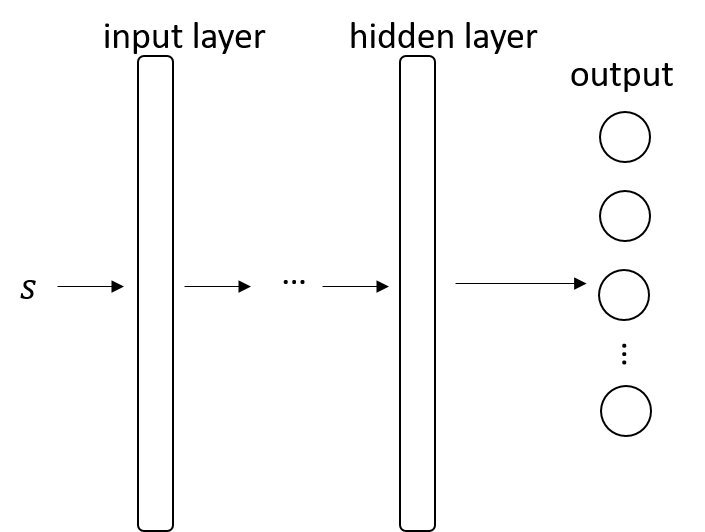
\includegraphics[width=0.5\linewidth]{../figures/optimalControl/reinforcementLearning/CanonicalDQN}
	\caption{The network architecture for canonical deep Q learning.}
	\label{fig:canonicaldqn}
\end{figure}

\begin{remark}[network archtecture]\hfill
\begin{itemize}
	\item The input is a high-dimensional state vector, the output is finite number of nodes. Each output (indexed by action $i$) represents the $Q$ value of taking action $i$. 
\end{itemize}	
	
\end{remark}


In the DQN framework, we use deep neutral network approximate the optimal action-value function
$$Q^{*}(s, a)=\max _{\pi} \mathbb{E}\left[r_{t}+\gamma r_{t+1}+\gamma^{2} r_{t+2}+\cdots | s_{t}=s, a_{t}=a, \pi\right],$$
which is maximizing accumulated discounted rewards in the process over all possible policy $\pi$ after achieving state $s$ and taking an action $a$, where $r_t$ is the one step reward function, $\gamma$ is the discount factor. 
With the optimal $Q*$, the optimal action at state $s$ is given by $a^* = \arg\max_{a} Q^*(s, a)$.  

Alternatively, using $\pi^*$ to denote the optimal policy $\pi^*(s) = \arg\max_{a} Q^*(s, a)$, we can re-write optimal $Q$ function by
$$Q^*(s, a) = \mathbb{E}\left[r_{t}+\gamma r_{t+1}+\gamma^{2} r_{t+2}+\cdots | s_{t}=s, a_{t}=a, \pi^*\right],$$
which is further connected to optimal state-value function by
$$V^*(s) = \mathbb{E}\left[r_{t}+\gamma r_{t+1}+\gamma^{2} r_{t+2}+\cdots | s_{t}=s, \pi^*\right] = \max_{a} Q^*(s, a).$$



Algorithm is from \cite{mnih2015human}

\begin{algorithm}

	Initialize replay memory $\cB$ to capacity $N$.\\
	Initialize action-value function $Q$ with random weights $\theta$.\\
	Initialize target action-value function $Q'$ with weights $\theta^- = \theta$. \\
	\For{ episode = 1, M}{
		Initialize sequence $s_1 = \{x_1\}$. \\
		\For{ $t = 1,T$}{
			With probability $\epsilon$ select a random action $a_t$, otherwise select $a_t = \arg\max_a Q(s_t, a; \theta)$. \\
			Execute action $a_t$ in emulator and observe reward $r_t$ and state $x_{t+1}$. \\
			Set $s_{t+1} = s_t, a_t, x_{t+1}$ and preprocess $s_{t+1}$.\\
			Store transition $(s_t,a_t,r_t,s_{t+1})$ in $\cB$.\\
			Sample random minibatch of transitions $(s_j,a_j,r_j,s_{j+1})$ from $\cB$. \\
			
			Set 
			$$y_j = \begin{cases*}
			r_j, \text{if episode terminates at step} j+1 \\
			r_j + \gamma \max_{a'}Q'(s_{j+1},a';\theta^-), \text{otherwise}
			\end{cases*}$$
			Every $C$ steps reset $Q' = Q$. 
		}
	}
	\caption{Deep Q-learning with experience replay}
\end{algorithm}

\begin{remark}[procedures to improve the stability of training]
	\begin{itemize}
		\item Before deep Q learning, target value used to train $Q$ network was
		$$r_j + \gamma \max_{a'}Q(s_{j+1},a';\theta),$$
		which leads to unstable training process. In deep Q learning, the target use is generated by a target network $Q'$, whose parameters are slowly updated, given by,
		$$r_j + \gamma \max_{a'}Q'(s_{j+1},a';\theta^-).$$
		\item Before deep Q learning, directly using consecutively generated samples also cause instability in the training process. This is because these samples are correlated and correlated samples applied to stochastic gradient method can lead to divergence. By using a replay buffer to randomly sample experience to learn, we decorrelate the sample and reuse samples.
		\item A helpful trick is to clip the error term
		$$y -  Q(s,a;\theta)$$
		between $[-1,1]$ or other more proper intervals. Such clipping corresponding to a more robust error function, like Huber loss function.  
	\end{itemize}
\end{remark}






\subsection{DQN variants}

\subsubsection{Overview}

Although Deep Q learning algorithm has achieved remarkable performance on various challenging tasks, there has been extensive discussion on its possible weaknesses? 

For example, 
\begin{itemize}
	\item The Q value is calculated using bootstrapped approach. Is such method accurate or biased?
	\item Is random sampling of experience is best option? Some experiences might be more important in contributing to the learning processes.
	\item Q network is directly learning state-action function. Will it be better to learn state value and action value separately?
	\item Is there any better approach to explore the state space beside $\epsilon$ greedy approach.
	\item The network structure is not suitable to handle tasks with long memory state dynamics. How to equip Q network with RNN structure?
	\item Deep Q learning usually takes a long time to converge.    
\end{itemize} 

Since the invention of the Deep Q learning algorithm, there have been various approaches to improve the canonical Deep Q learning algorithm (\href{https://zhuanlan.zhihu.com/p/21547911}{link}).


\subsubsection{Double Q learning}

In the canonical deep Q learning, 
$$y_t^{Q} = r_{t+1} + \gamma \max_{a'}Q'(\phi_{j+1},a';\theta^-),$$
the maximization operator can proporgate noise and overestimate Q values. 
In double Q-learning (\cite{van2016deep}), we use two networks to generate the target value
$$y_t^{DoubleQ} = r_{t+1} + \gamma Q'(s_{t+1}, \arg\max_{a}Q(s_{t+1},a;\theta_t);\theta_t')$$
where $Q'$ is used to generate target and $Q$ is used to generate action. 


\begin{algorithm}
	\KwIn{minibatch $k$, step-size $\eta$, replay period $K$ and size $N$, exponents $\alpha$ and $\beta$, budget $T$}
	Initialize replay memory $\cB = \emptyset$, $\Delta = 0, p_1 = 1$.\\
	Initialize action-value function $Q$ with random weights $\theta$.\\
	Initialize target action-value function $Q'$ with weights $\theta^- = \theta$. \\
	\For{ episode = 1, M}{
		Initialize sequence $s_1 = \{x_1\}$. \\
		\For{ $t = 1,T$}{
			With probability $\epsilon$ select a random action $a_t$, otherwise select $a_t = \arg\max_a Q(s_t, a; \theta)$. \\
			Execute action $a_t$ in emulator and observe reward $r_t$ and state $x_{t+1}$. \\
			Set $s_{t+1} = s_t, a_t, x_{t+1}$ and preprocess $s_{t+1}$.\\
			Store transition $(s_t,a_t,r_t,s_{t+1})$ in $\cB$.\\
			Sample random minibatch of transitions $(s_j,a_j,r_j,s_{j+1})$ from $\cB$. \\
			
			Define $a^* = \arg\max_{a}Q(s_{t+1},a;\theta_t)$. Set 
			$$y_j = \begin{cases*}
			r_j, \text{if episode terminates at step} j+1 \\
			r_j + \gamma Q'(s_{j+1},a^*;\theta^-), \text{otherwise}
			\end{cases*}$$
			Every $C$ steps reset $Q' = Q$. 
		}
	}
	\caption{Double Deep Q-learning with experience replay}
\end{algorithm}


Sample transition $j \sim P(j) = \frac{p_j^\alpha}{\sum_{i=1}^{N} p_i^\alpha}$. \\
Compute importance-sampling weight $w_j = (N\cdot P(j))$


\subsubsection{Double Q with prioritized experience replay}


\begin{algorithm}
	\KwIn{A randomly initialized critic network $Q(s,a|\theta^Q)$ and an actor network $\mu(s|\theta^\mu)$ with weights $\theta^Q,\theta^\mu$.}
	\KwOut{Optimal critic and actor networks}
	Initialize replay memory $\cB$ to capacity $N$.\\
	Initialize action-value function $Q$ with random weights $\theta$.\\
	Initialize target action-value function $Q'$ with weights $\theta^- = \theta$. \\
	\For{ episode = 1, M}{
		Initialize sequence $s_1 = \{x_1\}$ and preprocessed sequence $\phi_1 = \phi(s_1)$. \\
		\For{ $t = 1,T$}{
			With probability $\epsilon$ select a random action $a_t$, otherwise select $a_t = \arg\max_a Q(\phi(s_t), a; \theta)$. \\
			Execute action $a_t$ in emulator and observe reward $r_t$ and image $x_{t+1}$. \\
			Set $s_{t+1} = s_t, a_t, x_{t+1}$ and preprocess $\phi_{t+1} = \phi(s_{t+1})$.\\
			Store transition $(\phi_t,a_t,r_t,\phi_{t+1})$ in $\cB$.\\
			Sample random minibatch of transitions $(\phi_j,a_j,r_j,\phi_{j+1})$ from $\cB$. \\
			
			Set 
			$$y_j = \begin{cases*}
			r_j, \text{if episode terminates at step} j+1 \\
			r_j + \gamma \max_{a'}Q'(\phi_{j+1},a';\theta^-), \text{otherwise}
			\end{cases*}$$
			Every $C$ steps reset $Q' = Q$. 
		}
	}
	\caption{Deep Q-learning with experience replay}
\end{algorithm}








\subsubsection{Dueling network}




\subsubsection{Deep Recurrent Q-Learning }

\cite{hausknecht2015deep}


\subsubsection{Asynchronous Methods}
\cite{mnih2016asynchronous}


\begin{algorithm}
	\KwIn{minibatch $k$, step-size $\eta$, replay period $K$ and size $N$, exponents $\alpha$ and $\beta$, budget $T$}
	For each thread, initialize thresh step counter $t = 0$ \\
	Initialize target network parameters $\theta' = \theta$ \\
	Get initial state $s$
	\Repeat{ episode = 1, M}{
		With probability $\epsilon$ select a random action $a_t$, otherwise select $a_t = \arg\max_a Q(s_t, a; \theta)$. \\
		Execute action $a_t$ and observe reward $r_t$ and state $x_{t+1}$. \\
		Set $s_{t+1} = s_t, a_t, x_{t+1}$.\\
		 Set 
			$$y_j = \begin{cases*}
			r_j, \text{if episode terminates at step} j+1 \\
			r_j + \gamma \arg\max_a Q(s_{j+1},a^*;\theta'), \text{otherwise}
			\end{cases*}$$
		
		Every $C$ steps reset $Q' = Q$. 
	}
	
	\caption{Asynchronous Deep Q-Learning for each thread}
\end{algorithm}


\begin{remark}[interpretation]
\begin{itemize}
	\item Since agents are running different exploration policies at different state sub-regions, experiences are less likely to be correlated. Hence a replay memory is not necessary.
	\item No lock is used when update  
\end{itemize}
	
\end{remark}


\subsection{Hierachical deep Q learning}


\begin{remark}\cite{kulkarni2016hierarchical}
	
\end{remark}


\begin{align*}
Q_{1}^{*}(s, a ; g)&=\max _{\pi_{a g}} \mathrm{E}\left[\sum_{t^{\prime}=t}^{\infty} \gamma^{t^{\prime}-t} r_{t^{\prime}} | s_{t}=s, a_{t}=a, g_{t}=g, \pi_{a g}\right] \\
&=\max _{\pi_{a g}} \mathrm{E}\left[r_{t}+\gamma \max _{a_{t+1}} Q_{1}^{*}\left(s_{t+1}, a_{t+1} ; g\right) | s_{t}=s, a_{t}=a, g_{t}=g, \pi_{a g}\right]
\end{align*}

where g is the agent's goal in state s and $\pi_{ag}$ is the action policy.

$$Q_{2}^{*}(s, g)=\max _{\pi_{g}} \mathrm{E}\left[\sum_{t^{\prime}=t}^{t+N} f_{t^{\prime}}+\gamma \max _{g^{\prime}} Q_{2}^{*}\left(s_{t+N}, g^{\prime}\right) | s_{t}=s, g_{t}=g, \pi_{g}\right]$$
where $N$ denotes the number of time steps until low-level controller halts with current goal, $g'$ is the agent's goal in state $s_{t+N}$, and $\pi_g$ is the policy for selecting goals. Note that the dynamics $(s_t, g_t, f_t, s_{t+N})$ associated with $Q_2$ occurs at a time scale much faster than the transitions $(s_t, a_t, g_t, r_t, s_{t+1})$ associated with $Q_1$.


\subsection{Deterministic policy gradient algorithm}
\cite{silver2014deterministic}


In the stochastic policy gradient (SPG) approach, the action function is a parameterized probability distribution over the action space given by
$$\pi_{\theta}(a|s),$$
where $\theta$ is the parameter of the distribution, $a\in \cA$ is the action, and $s\in \cS$ is the state.

Deterministic policy gradient (DPG) approach differs from SPG in the following aspects:
\begin{itemize}
	\item It will map a state $s$ deterministically to an action $a$.
	\item DPG can be viewed as a special case of SPG where action variance is zero.
	\item 
\end{itemize}


\subsection{Deep deterministic policy gradient (DDPG) algorithm}

\begin{remark}[motivation]
	\begin{itemize}
		\item Deep Q network solves problems with high-dimensional observation space and it can only handle discrete and low dimensional action spaces.
		\item DDPG is developed to cope with both high-dimensional observation space and continuous, high dimensional action space. 
	\end{itemize}
\end{remark}



\begin{algorithm}
	\KwIn{A randomly initialized critic network $Q(s,a|\theta^Q)$ and an actor network $\mu(s|\theta^\mu)$ with weights $\theta^Q,\theta^\mu$.}
	\KwOut{Optimal critic and actor networks}
	Initialize target networks $Q'$ and $\mu'$ with weights $\theta^{Q'} = \theta^Q$ and $\theta^{\mu'} = \theta^\mu$. \\
	Initialize replay buffer $\cB$.
	Initialize policy parameter $\theta\in \R^d, w\in \R^m$\\
	\Repeat{ sufficient iterations}{
		Initialize a random process $\cN$ for action exploration. \\
		Initialize initial state $s_1$.\\
		\For{ $t = 1,T$}{
			Select action $a_t = \mu(s_t|\theta^\mu) + \cN_t$ according to current actor network and exploration noise.\\
			Execute action $a_t$ and observe reward $r_t$ and new state $s_{t+1}$. \\
			Store transition $(s_t,a_t,r_t,s_{t+1})$ in $\cB$.\\
			Sample a random minibatch of $N$ transitions $(s_i,a_i,r_i,s_{i+1})$ from $\cB$.\\
			Set $y_i = r_i + \gamma Q'(s_{i+1},\mu'(s_{i+1}|\theta^{\mu'})|\theta^{Q'})$. \\
			Update the critic network by minimizing the loss $$L = \frac{1}{N}\sum_{i}^N (y_i - Q(s_i,a_i|\theta^Q))^2.$$
			Update the actor policy network using the sampled policy graident:
			$$\nabla_{\theta^\mu} J \approx \frac{1}{N}\sum_{i=1}^N \nabla_a Q(s,a|\theta^Q)|_{s=s_i,a=\mu(s_i)}\nabla_{\theta^\mu}\mu(s|\theta^\mu)|_{s_i}.$$
			
			Update the target network
			$$\theta^{Q'} = \tau \theta^Q + (1-\tau)\theta^{Q'}$$ 
			$$\theta^{\mu'} = \tau \theta^Q + (1-\tau)\theta^{\mu'}$$
		}
	}
	\caption{Deep deterministic policy gradient algorithm}
\end{algorithm}

\begin{remark}[interpretation]DDPG (\cite{lillicrap2015continuous}) uses several techniques from DQN network(\cite{mnih2015human}) and double Q network (\cite{van2016deep}):
	\begin{itemize}
		\item experience replay to increase sample efficiency.
		\item target network $Q'$ and $\mu'$ to stabilize the training process. 
		\item 
	\end{itemize}
	
\end{remark}



\begin{remark}[implementation details]
	\begin{itemize}
		\item 
	\end{itemize}	
\end{remark}


\subsection{TD3}
The Q-learning algorithm is commonly known to suffer from the overestimation of the value function. This overestimation can propagate through the training iterations and negatively affect the policy. This property directly motivated Double Q-learning and Double DQN: the action selection and Q-value update are decoupled by using two value networks.

Twin Delayed Deep Deterministic (short for TD3; Fujimoto et al., 2018) applied a couple of tricks on DDPG to prevent the overestimation of the value function:

(1) Clipped Double Q-learning: In Double Q-Learning, the action selection and Q-value estimation are made by two networks separately. In the DDPG setting, given two deterministic actors (μθ1,μθ2) with two corresponding critics (Qw1,Qw2), the Double Q-learning Bellman targets look like:
However, due to the slow changing policy, these two networks could be too similar to make independent decisions. The Clipped Double Q-learning instead uses the minimum estimation among two so as to favor underestimation bias which is hard to propagate through training:

\begin{align*}
y_{1}&=r+\gamma \min _{i=1,2} Q_{w_{i}}\left(s^{\prime}, \mu_{\theta_{1}}\left(s^{\prime}\right)\right) \\
 y_{2}&=r+\gamma \min _{i=1,2} Q_{w_{i}}\left(s^{\prime}, \mu_{\theta_{2}}\left(s^{\prime}\right)\right)
\end{align*}

(2) Delayed update of Target and Policy Networks: In the actor-critic model, policy and value updates are deeply coupled: Value estimates diverge through overestimation when the policy is poor, and the policy will become poor if the value estimate itself is inaccurate.

To reduce the variance, TD3 updates the policy at a lower frequency than the Q-function. The policy network stays the same until the value error is small enough after several updates. The idea is similar to how the periodically-updated target network stay as a stable objective in DQN.

(3) Target Policy Smoothing: Given a concern with deterministic policies that they can overfit to narrow peaks in the value function, TD3 introduced a smoothing regularization strategy on the value function: adding a small amount of clipped random noises to the selected action and averaging over mini-batches.

\begin{align*}y&=r+\gamma Q_{w}\left(s^{\prime}, \mu_{\theta}\left(s^{\prime}\right)+\epsilon\right) \\ 
\epsilon &\sim \operatorname{clip}(\mathcal{N}(0, \sigma),-c,+c)
\end{align*}

clipped random noises.
This approach mimics the idea of SARSA update and enforces that similar actions should have similar values.


\begin{algorithm}
	\KwIn{A randomly initialized critic network $Q(s,a|\theta^Q)$ and an actor network $\mu(s|\theta^\mu)$ with weights $\theta^Q,\theta^\mu$.}
	\KwOut{Optimal critic and actor networks}
	Initialize target networks $Q'$ and $\mu'$ with weights $\theta^{Q'} = \theta^Q$ and $\theta^{\mu'} = \theta^\mu$. \\
	Initialize replay buffer $\cB$.
	Initialize policy parameter $\theta\in \R^d, w\in \R^m$\\
	\Repeat{ sufficient iterations}{
		Initialize a random process $\cN$ for action exploration. \\
		Initialize initial state $s_1$.\\
		\For{ $t = 1,T$}{
			Select action $a_t = \mu(s_t|\theta^\mu) + \cN_t$ according to current actor network and exploration noise.\\
			Execute action $a_t$ and observe reward $r_t$ and new state $s_{t+1}$. \\
			Store transition $(s_t,a_t,r_t,s_{t+1})$ in $\cB$.\\
			Sample a random minibatch of $N$ transitions $(s_i,a_i,r_i,s_{i+1})$ from $\cB$.\\
			Set $y_i = r_i + \gamma Q'(s_{i+1},\mu'(s_{i+1}|\theta^{\mu'})|\theta^{Q'})$. \\
			Update the critic network by minimizing the loss $$L = \frac{1}{N}\sum_{i}^N (y_i - Q(s_i,a_i|\theta^Q))^2.$$
			Update the actor policy network using the sampled policy graident:
			$$\nabla_{\theta^\mu} J \approx \frac{1}{N}\sum_{i=1}^N \nabla_a Q(s,a|\theta^Q)|_{s=s_i,a=\mu(s_i)}\nabla_{\theta^\mu}\mu(s|\theta^\mu)|_{s_i}.$$
			
			Update the target network
			$$\theta^{Q'} = \tau \theta^Q + (1-\tau)\theta^{Q'}$$ 
			$$\theta^{\mu'} = \tau \theta^Q + (1-\tau)\theta^{\mu'}$$
		}
	}
	\caption{Deep deterministic policy gradient algorithm}
\end{algorithm}

\section{Algorithm summary}

\begin{remark}\hfill
\begin{itemize}
	\item For large state space $\cS$, it can take a lot of iteration to converge. 
	\item Changes of $V(s)$ will be started at states that leads to states with nonzero rewards $r$. Then the changes will spread out.
\end{itemize}	
	
\end{remark}




\begin{remark}\hfill
	\begin{itemize}
		\item Here we assume the value function (associated with a policy, not necessarily the optimal policy) is known. And the summation over $r$ and $s$ can calculate $Q(s,a)$.
	\end{itemize}	
	
\end{remark}




\section{Temporal-Difference Methods}

%%%%%%%%%%%% 15 Expected Sarsa
\begin{algorithm}
	\KwIn{policy $\pi$, positive integer $num\_episodes$, small positive fraction $\alpha$, GLIE $\{\epsilon_i\}$}
	\KwOut{value function $Q$ ($\approx q_\pi$ if $num\_episodes$ is large enough)}
	Initialize $Q$ arbitrarily (e.g., $Q(s,a) = 0$ for all $s\in\mathcal{S}$ and $a\in\mathcal{A}(s)$, and $Q(terminal\text{-}state, \cdot)=0$) \\
	\For{$i \leftarrow 1 \textbf{ to } num\_episodes$}{
		$\epsilon \leftarrow \epsilon_i$\\
		Observe $S_0$\\
		$t\leftarrow 0$\\
		\Repeat{$S_t$ is terminal}{
			Choose action $A_t$ using policy derived from $Q$ (e.g., $\epsilon$-greedy)\\
			Take action $A_{t}$ and observe $R_{t+1}, S_{t+1}$\\
			$Q(S_t, A_t) \leftarrow Q(S_t, A_t) + \alpha (R_{t+1} + \gamma \sum_{a}\pi(a|S_{t+1})Q(S_{t+1}, a) - Q(S_t, A_t))$\\
			$t \leftarrow t+1$
		}
	}
	\KwRet{$Q$}
	\caption{Expected Sarsa}
\end{algorithm}


\section{Notes on bibliography}


For certainty equivalence, see \cite[160]{bertsekas2012dynamic}

For dynamic programming theory, see abstract dynamic programming.

For reinforcement learning, see \cite{wiering2012reinforcement}.

For applications in finance, see \cite{chang2004stochastic}\cite{pham2009continuous}\cite{bertsekas2012dynamic}.

Playing Atari with Deep Reinforcement Learning, Mnih et al., 2013 \\
Human-level control through deep reinforcement learning, Mnih et al., 2015 \\
Deep Reinforcement Learning with Double Q-learning, van Hasselt et al., 2015 \\
Continuous control with deep reinforcement learning, Lillicrap et al., 2015 \\
Asynchronous Methods for Deep Reinforcement Learning, Mnih et al., 2016 \\
Continuous Deep Q-Learning with Model-based Acceleration, Gu et al., 2016 \\
Learning Tetris Using the Noisy Cross-Entropy Method, Szita et al., 2006 \\
Deep Reinforcement Learning (MLSS lecture notes), Schulman, 2016 \\
Dueling Network Architectures for Deep Reinforcement Learning, Wang et al., 2016 \\
Reinforcement learning: An introduction, Sutton and Barto, 2011 \\
Proximal Policy Optimization Algorithms, Schulman et al., 2017 \\
\printbibliography

\end{refsection}